%% Copernicus Publications Manuscript Preparation Template for LaTeX Submissions
%% ---------------------------------
%% This template should be used for the following class files: copernicus.cls, copernicus2.cls, copernicus_discussions.cls
%% The class files, the Copernicus LaTeX Manual with detailed explanations regarding the comments
%% and some style files are bundled in the Copernicus Latex Package which can be downloaded from the different journal webpages.
%% For further assistance please contact the Publication Production Office (production@copernicus.org).
%% http://publications.copernicus.org


%% Differing commands regarding the specific class files are highlighted.


%% copernicus.cls
\documentclass[gmd]{copernicus}

% A few handy shortcuts
\newcommand{\uf}{\ensuremath{\widetilde{u}}}
\newcommand{\vf}{\ensuremath{\widetilde{v}}}
\newcommand{\thetaf}{\ensuremath{\widetilde{\theta}}}
\newcommand{\phif}{\ensuremath{\widetilde{\phi}}}

\begin{document}

\linenumbers
\raggedbottom

\title{MicroHH 1.0: a computational fluid dynamics code for direct and large-eddy simulation of atmospheric boundary layer flows}


\author[1,2]{Chiel C. van Heerwaarden}
\author[1,2]{Bart J. H. van Stratum}
\author[3]{Thijs Heus}
\author[4]{Jeremy A. Gibbs}
\author[4]{Evgeni Fedorovich}

\affil[1]{Meteorology and Air Quality Group, Wageningen University, Wageningen, The Netherlands}
\affil[2]{Max Planck Institute for Meteorology, Hamburg, Germany}
\affil[3]{Cleveland State University, Cleveland, OH, USA}
\affil[4]{University of Oklahoma, Norman, OK, USA}

%% The [] brackets identify the author to the corresponding affiliation, 1, 2, 3, etc. should be inserted.



\runningtitle{MicroHH 1.0}

\runningauthor{van Heerwaarden et al.}

\correspondence{Chiel van Heerwaarden\\ (chiel.vanheerwaarden@wur.nl)}



\received{}
\pubdiscuss{} %% only important for two-stage journals
\revised{}
\accepted{}
\published{}

%% These dates will be inserted by the Publication Production Office during the typesetting process.


\firstpage{1}

\maketitle  %% Please note that for the copernicus2.cls this command needs to be inserted after \abstract{TEXT}

\begin{abstract}
This paper describes MicroHH 1.0, a new and open source (\url{www.microhh.org}) Computational Fluid Dynamical code for the simulation of wall-bounded turbulent flows in the atmosphere using Direct Numerical Simulation and Large-Eddy Simulation. The paper covers the description of the governing equations, their numerical implementation, and the parametrizations involved in the code. Furthermore, the paper presents the validation of the dynamical core in the form of convergence tests and conservation tests and comparison of simulations of channel flows and slope flows against well-established test cases. The full numerical model, including the associated parametrizations for Large-Eddy Simulations of high Reynolds number flows, has been tested for a set of cases under stable and unstable conditions, under the Boussinesq and anelastic approximation and with dry and moist convection under stationary and time-varying boundary conditions. The paper presents performance tests showing good scaling from 256 to 32,768 processes. The Graphical Processing Unit-enabled version of the code reaches speedups of more than an order of magnitude with respect to the conventional code for a variety of cases.
\end{abstract}

\introduction  %% \introduction[modified heading if necessary]
In this paper we present a description of MicroHH 1.0, a new Computational Fluid Dynamical code for the simulation of wall-bounded turbulent flows, with a focus on those in the atmosphere. MicroHH can solve flows using the Direct Numerical Simulation (DNS) and Large-Eddy Simulation (LES) techniques, with applications ranging from neutral channel flows to cloud-covered atmospheric boundary layers on large-domains. The model has been designed and written from scratch with the aim of creating a highly parallel code that is able to run on more than 10,000 processes with the support of modern techniques. MicroHH has been written in C++ and CUDA, in contrast to the majority of its peers, which are mostly written in Fortran 90.

This paper is built up as following: in Section \ref{sec:dyncore}, we provide a full description of the governing equations of the dynamical core, and their numerical implementation is discussed in Section \ref{sec:dyncorediscrete}. Subsequently, in Section \ref{sec:parametrizations} we present the parameterizations and their underlying assumptions. Section \ref{sec:technical} discusses the technical details of the code. This is followed by a series of model tests on validity, accuracy, and performance in Section \ref{sec:tests}, followed by a series of test cases based on previous scientific research (Section \ref{sec:casestudies}). After a short description on how to download, compile and run MicroHH (Section \ref{sec:howto}), concluding remarks and future plans close the paper (Section \ref{sec:conclusion}). In order to keep the explanations of mathematical expressions concise, we have included an Appendix with the symbols, their description and  units.

\section{Dynamical core: governing equations}\label{sec:dyncore}
The dynamical core of MicroHH solves the conservation equations of mass, momentum and energy under the anelastic approximation \citep{Bannon1996}. Under this approximation, the state variables density, pressure and temperature are described as small fluctuations (denoted with a prime in this paper) around a vertical reference profile (denoted with subscript zero) that is a function of height only. This form of the approximation directly simplifies to the Boussinesq equations if the reference density $\rho_0$ is assumed to be constant with height $z$. To facilitate the subsequent discussion of the conservation equations, we define the scale height for density $H_\rho$ based on the reference density profile
\begin{eqnarray}
H_{\rho} & \equiv & \left( \dfrac{1}{\rho_0} \dfrac{d \rho_0}{dz} \right)^{-1}.
\end{eqnarray}

\subsection{Conservation of mass}
The conservation of mass is formulated as
\begin{eqnarray}
\dfrac{\partial \rho_0 u_i}{\partial x_i} & = & \rho_0 \dfrac{\partial u_i}{\partial x_i} + \rho_0 w H_{\rho}^{-1} = 0, \label{eq:consmassa}
\end{eqnarray}
where $u_i$ is the velocity vector $(u,v,w)$ and $x_i$ is the position vector $(x,y,z)$.
Under the Boussinesq approximation ($H_{\rho}~\rightarrow~\infty$), Eq. \ref{eq:consmassa} simplifies to conservation of volume
\begin{eqnarray}
\dfrac{\partial u_i}{\partial x_i} & = & 0. \label{eq:consmassb}
\end{eqnarray}

\subsection{Conservation of momentum and the equation of state}
The momentum equation is written in the flux form, in order to assure the best possible mass and momentum conservation. The hydrostatic balance $dp_0 / dz~=~-\rho_0 g$ has been subtracted to arrive at the perturbation form
\begin{eqnarray}
\nonumber \dfrac{\partial u_i}{\partial t} & = & - \dfrac{1}{\rho_0} \dfrac{\partial \rho_0 u_i u_j}{\partial x_j} 
- \dfrac{\partial}{\partial x_i}\left(\dfrac{p'}{\rho_0}\right) \\
& + & \delta_{i3} g \dfrac{\theta_v'}{\theta_{v0}} + \nu \dfrac{\partial^2 u_i}{\partial x_j^2} + F_i,\label{eq:consmoma}
\end{eqnarray}
where $p^\prime$ is the perturbation pressure, $\delta$ is the Kronecker delta, $g$ is the gravity acceleration, $\theta_v^\prime$ is the perturbation virtual potential temperature,  $\theta_{v0}$ the reference virtual potential temperature, $\nu$ the kinematic viscosity, and vector $F_i$ represents external forces resulting from parameterizations or large-scale forcings.

The corresponding equation of state is (see \citet{Bannon1996} for the derivation)
\begin{eqnarray}
\dfrac{\theta_v'}{\theta_{v0}} & = & \dfrac{p'}{\rho_0 g H_{\rho}} - \dfrac{\rho'}{\rho_0}.\label{eq:statea}
\end{eqnarray}

Under the Boussinesq approximation the two equations simplify to
\begin{eqnarray}
\nonumber \dfrac{\partial u_i}{\partial t} & = & - \dfrac{\partial u_i u_j}{\partial x_j} - \dfrac{1}{\rho_0}\dfrac{\partial p^\prime}{\partial x_i} \\
& + & \delta_{i3} g \dfrac{\theta_v'}{\theta_{v0}} + \nu \dfrac{\partial^2 u_i}{\partial x_j^2} + F_i \label{eq:consmomb},\\
\dfrac{\theta_v'}{\theta_{v0}} & = & - \dfrac{\rho'}{\rho_0}\label{eq:stateb}.
\end{eqnarray}

\subsection{Pressure equation}
The equation to acquire the pressure is diagnostic, because density fluctuations are neglected in the conservation of mass in the anelastic equations (Eq. \ref{eq:consmassa}). To simplify the notation, we define a function $f \left( u_i \right)$ that contains all right-hand side terms of Eq. \ref{eq:consmoma}, except the pressure gradient. To arrive at the equation that allows us to solve for the pressure, we multiply the equation with the base density $\rho_0$ and take its divergence. Conservation of mass ensures that the tendency term vanishes, and an elliptic equation for pressure remains
\begin{eqnarray}
\dfrac{\partial}{\partial x_i} 
\left[ \rho_0 \dfrac{\partial}{\partial x_i} \left( \dfrac{p'}{\rho_0} \right) \right] & = &
\dfrac{\partial \rho_0 f \left( u_i \right)}{\partial x_i}.\label{eq:presa}
\end{eqnarray}
Under the Boussinesq approximation the equation simplifies to
\begin{eqnarray}
\dfrac{\partial^2}{\partial x_i^2} \left( \dfrac{p'}{\rho_0} \right) & = &
\dfrac{\partial f \left( u_i \right)}{\partial x_i}.\label{eq:presb}
\end{eqnarray}
In Section \ref{sec:dyncorediscrete} we explain how these equations are solved.

\subsection{Conservation of an arbitrary scalar}
The conservation equation of an arbitrary scalar $\phi$ can be written in flux form:
\begin{eqnarray}
\dfrac{\partial \phi}{\partial t} & = & - \dfrac{1}{\rho_0} \dfrac{\partial \rho_0 u_j \phi}{\partial x_j} +
\kappa_\phi \dfrac{\partial^2 \phi}{\partial x_j^2} + S_\phi, \label{eq:consscal}
\end{eqnarray}
where $\kappa_\phi$ is the diffusivity of the scalar, and $S_\phi$ represents sources and sinks of the variable.

\subsection{Conservation of energy}
MicroHH provides multiple options for the energy conservation equation. Two modes work with potential temperature $\theta$ (dry dynamics) or liquid water potential temperature $\theta_l$ (moist dynamics) with the following conservation equation
\begin{eqnarray}
\dfrac{\partial \theta}{\partial t} & = & - \dfrac{1}{\rho_0} \dfrac{\partial \rho_0 u_j \theta}{\partial x_j} + \kappa_\phi \dfrac{\partial^2 \theta}{\partial x_j^2} + \dfrac{\theta_0}{\rho_0 c_p T_0} Q,
\end{eqnarray}
where $\kappa_\theta$ is the thermal diffusivity for heat, and $Q$ represents heating sources or sinks.

A third, more simplified mode, is available for dry dynamics under the Boussinesq approximation. Here, the equation of state can be eliminated and the conservation of momentum and energy can be written using buoyancy $b \equiv (g/\theta_0)\theta^\prime$ as
\begin{eqnarray}
\dfrac{\partial u_i}{\partial t} + \dfrac{\partial u_i u_j}{\partial x_j} & = & 
- \dfrac{1}{\rho_0}\dfrac{\partial p'}{\partial x_i} + \delta_{i3} b + \nu \dfrac{\partial^2 u_i}{\partial x_j^2}\label{eq:consmombsimp},\\
\dfrac{\partial b}{\partial t} + \dfrac{\partial b u_j}{\partial x_j} & = & 
\kappa_b \dfrac{\partial^2 b}{\partial x_j^2}\label{eq:consenbsimp}.
\end{eqnarray}
with $\kappa_b$ as the thermal diffusivity for buoyancy.

With a slight modification to the previous set of equations, it is possible to study slope flows in periodic domains. If we introduce a slope $\alpha$ in the x-direction, introduce the proper gravity vector, and subtract the background buoyancy profile $N^2 z$ from the buoyancy value, the set of Eqs. \ref{eq:consmombsimp} and \ref{eq:consenbsimp} becomes
\begin{eqnarray}
\dfrac{\partial u}{\partial t} + \dfrac{\partial u_j u}{\partial x_j} & = & 
- \dfrac{1}{\rho_0}\dfrac{\partial p'}{\partial x} + \sin(\alpha) b + \nu \dfrac{\partial^2 u}{\partial x_j^2}\label{eq:consuslope},\\
\dfrac{\partial w}{\partial t} + \dfrac{\partial u_j w}{\partial x_j} & = & 
- \dfrac{1}{\rho_0}\dfrac{\partial p'}{\partial z} + \cos(\alpha) b + \nu \dfrac{\partial^2 w}{\partial x_j^2}\label{eq:conswslope},\\
\dfrac{\partial b}{\partial t} + \dfrac{\partial b u_j}{\partial x_j} & = & 
\kappa_b \dfrac{\partial^2 b}{\partial x_j^2} - \left (u\,\sin(\alpha) + w\,\cos(\alpha) \right) N^2\label{eq:consbslope}
\end{eqnarray}
where the evolution equation of $v$ is omitted as it contains no changes.

\section{Dynamical core: numerical implementation}\label{sec:dyncorediscrete}
\subsection{Time integration}
The prognostic equations are solved using low-storage Runge-Kutta time integration schemes, where each prognostic variable requires only two three-dimensional fields. These we denote in this section with $\phi$ for an arbitrary prognostic variable and $\delta \phi$ for its tendency that is carried on during all stages of the time integration. The code provides two options: a three-stage third-order scheme \citep{Williamson1980} and a five-stage fourth-order scheme \citep{Carpenter1994}. Both can be written in the same generic form in semi-discrete formulation
\begin{eqnarray}
\left( \delta \phi \right)_n & = & f \left( \phi_n \right) + a_n \left( \delta \phi \right)_{n-1} \\
\phi_{n+1} & = & \phi_n + b_n \Delta t \left( \delta \phi \right)_{n},
\end{eqnarray}
where $f$ is a function that represents the computation of all right-hand side terms, $a_n$ and $b_n$ are the coefficients for the Runge-Kutta method at stage $n$, and $\Delta t$ is the time step. Expression $f \left( \phi_n \right)$ represents thus the actual tendency calculated using for instance Eqs. \ref{eq:consmoma} or \ref{eq:consscal}, whereas $(\delta \phi)_n$ is a composite of the actual tendency and those of the previous stages. In low-storage form, the tendencies of the previous stage $\left( \delta \phi \right)_{n-1}$ are retained and multiplied with $a_n$ at the beginning of a stage, except for the first stage, where $a_1 = 0$. 

For the third-order scheme the vectors $a_n$ and $b_n$ are
\begin{eqnarray}
a_n & = & \left\{0, -\frac{5}{9}, -\frac{153}{128} \right\}\\
b_n & = & \left\{\frac{1}{3}, \frac{15}{16}, \frac{8}{15} \right\}
\end{eqnarray}

For the fourth-order scheme the vectors $a$ and $b$ are
\begin{eqnarray}
\nonumber a_n & = & \left\{0, -\frac{567301805773}{1357537059087},
-\frac{2404267990393}{2016746695238},\right.\\
& & \left. -\frac{3550918686646}{2091501179385},
-\frac{1275806237668}{842570457699} \right\}\\
\nonumber b_n & = & \left\{\frac{1432997174477}{9575080441755}, \frac{5161836677717}{13612068292357},
\frac{1720146321549}{2090206949498},\right.\\
& & \left. \frac{3134564353537}{4481467310338},
\frac{2277821191437}{14882151754819} \right\}
\end{eqnarray}

The reduced truncation error of the fourth-order scheme makes the scheme preferable over the third-order scheme under many conditions (see Section \ref{sec:validationtime}).

\subsection{Grid}
MicroHH is discretized on a staggered Arakawa C-grid, where the scalars are located in the center of a grid cell and the three velocity components at the faces.

MicroHH can work with stretched grids in the vertical dimension. The grid is initialized from vertical profiles that give the location of the cell centres. The locations of the faces are determined consistent with the spatial order of the interpolations that are described in the next section.

\subsection{Building blocks of the spatial discretization}
The spatial operators are based on finite differences. The code supports second-order and fourth-order accurate discretizations following \citet{Morinishi1998, Vasilyev2000}. From Taylor series spatial operators can be derived that form the building blocks of more advanced operators, such as the advection and diffusion operators. In the following subsections we describe the operators and those that can be derived from them. We use only two dimensions for brevity.

We define two second-order interpolation operators, the former with a small stencil and the latter with a wide stencil
\begin{eqnarray}
\phi_{i,j} \approx \widehat{\phi}^{2x }_{i,j} & \equiv & \dfrac{\phi_{i-\frac{1}{2},j} + \phi_{i+\frac{1}{2},j}}{2},\\
\phi_{i,j} \approx \widehat{\phi}^{2xL}_{i,j} & \equiv & \dfrac{\phi_{i-\frac{3}{2},j} + \phi_{i+\frac{3}{2},j}}{2},
\end{eqnarray}
Interpolations are marked with a hat. The superscript indicates the spatial order (2), and the direction ($x$) and has an extra qualifier $L$ when it is taken over a greater distance. The subscript indicates the position on the grid ($i,j$).

The gradient operators, denoted with operator $\delta$, are defined in a similar way
\begin{eqnarray}
\left. \dfrac{\partial \phi}{\partial x}\right|_{i,j} \approx \delta^{2x} \left( \phi \right)_{i,j} & \equiv & \dfrac{\phi_{i+\frac{1}{2},j} - \phi_{i-\frac{1}{2},j}}
                                                                                                                 {   x_{i+\frac{1}{2}}   -    x_{i-\frac{1}{2}  }} \\
\left. \dfrac{\partial \phi}{\partial x}\right|_{i,j} \approx \delta^{2xL} \left( \phi \right)_{i,j}& \equiv & \dfrac{\phi_{i+\frac{3}{2},j} - \phi_{i-\frac{3}{2},j}}
                                                                                                                  {   x_{i+\frac{3}{2}}   -    x_{i-\frac{3}{2}  }}
\end{eqnarray}
We use the Einstein summation in the operators. For instance, the divergence of vector $\left.u_i\right|_{i,j}$ can be written as $\delta^{2x_i}\left( u_i \right)_{i,j}$.
% \begin{eqnarray}
% \delta^{2x} \left( \phi \right)_{i,j} = \dfrac{\phi_{i+\frac{1}{2},j} - \phi_{i-\frac{1}{2},j}}
%                                               {\Delta x}
% \end{eqnarray}
% 
% \begin{eqnarray}
% \delta^{2xL} \left( \phi \right)_{i,j} = \dfrac{\phi_{i+\frac{3}{2},j} - \phi_{i-\frac{3}{2},j}}
%                                                {3\Delta x}
% \end{eqnarray}

The fourth-order operators, written down in the same notation, are defined as
\begin{eqnarray}
\phi_{i,j} \approx \widehat{\phi}^{4x}_{i,j} \equiv \dfrac{- \phi_{i-\frac{3}{2},j} + 9 \phi_{i-\frac{1}{2},j} + 9 \phi_{i+\frac{1}{2},j} - \phi_{i+\frac{3}{2},j}}{16},\label{eq:interp4}
\end{eqnarray}
and a biased one that can by applied in the vicinity of the boundaries. Note that we only write down the bottom boundary (marked with superscript qualifier $b$) for brevity
\begin{eqnarray}
\phi_{i,j} \approx \widehat{\phi}^{4xb}_{i,j} \equiv \dfrac{ 5 \phi_{i-\frac{1}{2},j} + 15 \phi_{i+\frac{1}{2},j} - 5 \phi_{i+\frac{3}{2},j} + \phi_{i+\frac{5}{2},j}}{16}.
\end{eqnarray}

The centered and biased fourth-order gradient operators are
\begin{eqnarray}
\nonumber
\left. \dfrac{\partial \phi}{\partial x}\right|_{i,j} & \approx & \delta^{4x} \left( \phi \right)_{i,j}\\
& \equiv & \dfrac{\phi_{i-\frac{3}{2},j} - 27 \phi_{i-\frac{1}{2},j} + 27 \phi_{i+\frac{1}{2},j} - \phi_{i+\frac{3}{2},j}}
             {       x_{i-\frac{3}{2}}   - 27    x_{i-\frac{1}{2}}   + 27    x_{i+\frac{1}{2}}   -    x_{i+\frac{3}{2}}},
\end{eqnarray}
and

\begin{eqnarray}
\nonumber
\left. \dfrac{\partial \phi}{\partial x}\right|_{i,j} & \approx & \delta^{4xb} \left( \phi \right)_{i,j}\\
& \equiv & \dfrac{-23 \phi_{i-\frac{1}{2},j} + 21 \phi_{i+\frac{1}{2},j} + 3 \phi_{i+\frac{3}{2},j} - \phi_{i+\frac{5}{2},j}}
                 {-23    x_{i-\frac{1}{2}}   + 21    x_{i+\frac{1}{2}}   + 3    x_{i+\frac{3}{2}}   -    x_{i+\frac{5}{2}}}
\end{eqnarray}

% \begin{eqnarray}
% \delta^{4x} \left( \phi \right)_{i,j}  = \dfrac{\phi_{i-\frac{3}{2},j} - 27 \phi_{i-\frac{1}{2},j} + 27 \phi_{i+\frac{1}{2},j} - \phi_{i+\frac{3}{2},j}}
%                                                {24 \Delta x}
% \end{eqnarray}

% \begin{eqnarray}
% \nonumber 
% &&\left. \dfrac{\partial^2 \phi}{\partial x^2}\right|_{i,j} \approx \delta^{4x} \left( \delta^{4x} \left( \phi \right) \right)_{i,j}\\
% \nonumber
% && = \dfrac{1}{576 \left( \Delta x \right)^2} \left( \phi_{i-3,j} - 54 \phi_{i-2,j} + 783 \phi_{i-1,j}\right.\\
% &&  \left. - 1460  \phi_{i,j} + 783 \phi_{i+1,j} - 54 \phi_{i+2,j} + \phi_{i+3,j} \right)
% \end{eqnarray}

\subsection{Advection}
We use the previously introduced notation to describe the more complex operators and expand them for illustration. The advection term is discretized in the flux form, where $\phi$ is an arbitrary scalar located in the center of the grid cell. In second order, this gives the following discretization
\begin{eqnarray}
\nonumber
\left. \dfrac{\partial u \phi}{\partial x}\right|_{i,j} + \left. \dfrac{\partial v \phi}{\partial y} \right|_{i,j} & \approx & 
\delta^{2x} \left( u \widehat{\phi}^{2x} \right)_{i,j} + \delta^{2y} \left( u \widehat{\phi}^{2y} \right)_{i,j} \\ 
& = & \dfrac{ u_{i+\frac{1}{2},j} \widehat{\phi}^{2x}_{i+\frac{1}{2},j} - u_{i-\frac{1}{2},j} \widehat{\phi}^{2x}_{i-\frac{1}{2},j} }
            { x_{i+\frac{1}{2}} - x_{i-\frac{1}{2}} }\\
& + & \dfrac{ v_{i,j+\frac{1}{2}} \widehat{\phi}^{2y}_{i,j+\frac{1}{2}} - v_{i,j-\frac{1}{2}} \widehat{\phi}^{2y}_{i,j-\frac{1}{2}} }
            { y_{j+\frac{1}{2}} - y_{j-\frac{1}{2}} }
\end{eqnarray}
The discretization of the advection of the velocity components (see Eqs. \ref{eq:consmoma} and \ref{eq:consmomb}) involves extra interpolations as the following example illustrates
\begin{eqnarray}
\left. \dfrac{\partial v u}{\partial x} \right|_{i,j} & = & \delta^{2x} \left( \widehat{v}^{2y} \widehat{u}^{2x} \right)_{i,j} \\
& = & \dfrac{ \widehat{v}^{2y}_{i+\frac{1}{2},j} \widehat{u}^{2x}_{i+\frac{1}{2},j} - \widehat{v}^{2y}_{i-\frac{1}{2},j} \widehat{u}^{2x}_{i-\frac{1}{2},j} }
      { x_{i+\frac{1}{2}} - x_{i-\frac{1}{2}} }\label{eq:advec2u}
\end{eqnarray}
In the standard fourth-order scheme, the scalar advection in flux form is denoted as
\begin{eqnarray}
\nonumber
\left. \dfrac{\partial u \phi}{\partial x} \right|_{i,j} & \approx & \delta^{4x} \left( u \widehat{\phi}^{4x} \right)_{i,j} \\
\nonumber
& = & \left( u_{i-\frac{3}{2},j} \widehat{\phi}^{4x}_{i-\frac{3}{2},j} - 27 u_{i-\frac{1}{2},j} \widehat{\phi}^{4x}_{i-\frac{1}{2},j} \right.\\
\nonumber
&   &\left. + 27 u_{i+\frac{1}{2},j} \widehat{\phi}^{4x}_{i+\frac{1}{2},j} - u_{i+\frac{3}{2},j} \widehat{\phi}^{4x}_{i+\frac{3}{2},j} \right)\\
&   &\slash \left( x_{i-\frac{3}{2}} - 27 x_{i-\frac{1}{2}} + 27 x_{i+\frac{1}{2}} - x_{i+\frac{3}{2}} \right).
\end{eqnarray}
Hereafter, we assume that operator notation is clear and only expand them where necessary.

MicroHH has fully energy-conserving fourth-order advection schemes \citep{Morinishi1998} available. These consist of interpolation of two energy conserving second-order schemes to eliminate the second-order error
\begin{eqnarray}
% \nonumber
\left. \dfrac{\partial u \phi}{\partial x} \right|_{i,j} & = & \frac{9}{8} \delta^{2x} \left( u \widehat{\phi}^{2x} \right)_{i,j} 
                                                             - \frac{1}{8} \delta^{2xL} \left( u \widehat{\phi}^{2xL} \right)_{i,j}%\\
% \nonumber
% & = & \frac{9}{16} \dfrac{ u_{i+\frac{1}{2},j} \widehat{\phi}^x_{i+\frac{1}{2},j} - u_{i-\frac{1}{2},j} \widehat{\phi}^x_{i-\frac{1}{2},j} }
%                           { x_{i+\frac{1}{2}} - x_{i-\frac{1}{2}} }\\
% & - & \frac{1}{16} \dfrac{ u_{i+\frac{3}{2},j} \widehat{\phi}^{3x}_{i+\frac{3}{2},j} - u_{i-\frac{3}{2},j} \widehat{\phi}^{3x}_{i-\frac{3}{2},j} }
%                           { x_{i+\frac{3}{2}} - x_{i-\frac{3}{2}} }
\end{eqnarray}
Velocity interpolations, such as those in Eq. \ref{eq:advec2u}, still need to be performed with fourth-order accuracy (Eq. \ref{eq:interp4}) in order to  be fourth-order accurate (see \citet{Morinishi1998} for details). The expression
\begin{eqnarray}
\dfrac{\partial v u}{\partial x} \approx \frac{9}{8} \delta^{2x} \left( \widehat{v}^{4y} \widehat{u}^{2x} \right)_{i,j} 
                                       - \frac{1}{8} \delta^{2xL} \left( \widehat{v}^{4y} \widehat{u}^{2xL} \right)_{i,j}
\end{eqnarray}
has for instance a combination of second- and fourth-order interpolations.

\subsection{Diffusion}
We use a mimetic discretization for the diffusion that can be written as the divergence of a gradient, using the building blocks defined earlier in this section. As this operator is identical in all directions, we write down only one dimension
\begin{eqnarray}
\left. \kappa_\phi \dfrac{\partial^2 \phi}{\partial x^2}\right|_{i,j} & \approx &
\kappa_\phi \delta^{2x} \left( \delta^{2x} \left( \phi \right) \right)_{i,j}\\
% \kappa_\phi \dfrac{\left. \dfrac{\partial \phi}{\partial x}\right|_{i+\frac{1}{2},j} - \left. \dfrac{\partial \phi}{\partial x}\right|_{i-\frac{1}{2},j}}
%                                 {   x_{i+\frac{1}{2},j} -    x_{i-\frac{1}{2},j}}
\left. \kappa_\phi \dfrac{\partial^2 \phi}{\partial x^2}\right|_{i,j} & \approx &
\kappa_\phi \delta^{4x} \left( \delta^{4x} \left( \phi \right) \right)_{i,j}
\end{eqnarray}

On an equidistant grid, this leads to the well-known second-order accurate operator for the second derivative
\begin{eqnarray}
\kappa_\phi \delta^{2x} \left( \delta^{2x} \left( \phi \right) \right)_{i,j} =
\kappa_\phi \dfrac{ \phi_{i-1,j} - 2 \phi_{i,j} + \phi_{i+1,j} }{\left( \Delta x \right)^2},
\end{eqnarray}
where $\Delta x$ is the uniform grid spacing.

For a fourth-order accurate operator, a seven-point stencil is derived
\begin{eqnarray}
\nonumber
&& \kappa_\phi \delta^{4x} \left( \delta^{4x} \left( \phi \right) \right)_{i,j}\\
\nonumber
&& = \dfrac{\kappa_\phi}{576 \left( \Delta x \right)^2} \left( \phi_{i-3,j} - 54 \phi_{i-2,j} + 783 \phi_{i-1,j}\right.\\
&&  \left. - 1460  \phi_{i,j} + 783 \phi_{i+1,j} - 54 \phi_{i+2,j} + \phi_{i+3,j} \right).
\end{eqnarray}
The seven point wide stencil and its properties has been discussed in detail in \citet{Castillo1995}.
% \begin{eqnarray}
% \nonumber
% \left. \kappa_\phi \dfrac{\partial^2 \phi}{\partial x^2}\right|_{i,j} & = & \kappa_\phi
% \left( \left. \dfrac{\partial \phi}{\partial x}\right|_{i-\frac{3}{2},j} 
% - 27 \left. \dfrac{\partial \phi}{\partial x}\right|_{i-\frac{1}{2},j} \right. \\
% \nonumber
% & & \left. + 27 \left. \dfrac{\partial \phi}{\partial x}\right|_{i+\frac{1}{2},j} 
% - \left. \dfrac{\partial \phi}{\partial x}\right|_{i+\frac{3}{2},j} \right)\\
% & & / \left( x_{i-\frac{3}{2}} - 27    x_{i-\frac{1}{2}} + 27    x_{i+\frac{1}{2}} -    x_{i+\frac{3}{2}} \right)
% \end{eqnarray}
\subsection{Pressure}
The pressure solver has to solve Eqs. \ref{eq:presa} and \ref{eq:presb} following the method of \citet{Chorin1968}. This method is a fractional step method that first computes an intermediate velocity component for the next time step based on all right hand side terms of the momentum conservation equation Eq. \ref{eq:consmoma}, denoted with a tilde
\begin{eqnarray}
\left. \widetilde{u_i} \right|^{t+1}_{i,j,k} & = & \left. u_i \right|^{t}_{i,j,k} + \Delta t \left. f_i \right|^{t}_{i,j,k}
\end{eqnarray}
The value at the next time step can be computed as soon as the pressure is known with
\begin{eqnarray}
\left. u_i\right|^{t+1}_{i,j,k} & = & \left. \widetilde{u_i} \right|^{t+1}_{i,j,k} - \Delta t \left. \delta^{nx_i}\left( \dfrac{p}{\rho_0}\right)\right|^t_{i,j,k}
\end{eqnarray}
In order to compute the pressure, we multiply the previous equation with the reference density and take its gradient, to arrive at
\begin{eqnarray}
\nonumber \left. \delta^{nx_i} \left( \rho_0 u_i\right) \right|^{t+1}_{i,j,k} & = & 
\left. \delta^{nx_i} \left( \rho_0 \widetilde{u_i} \right) \right|^{t+1}_{i,j,k}\\
& - &  \Delta t \left.\delta^{nx_i} \left[ \rho_0 \delta^{nx_i}\left( \dfrac{p}{\rho_0}\right) \right] \right|^t_{i,j,k}
\end{eqnarray}
The left hand side is the conservation of mass at the next time step, which equals zero (Eq. \ref{eq:consmassa}). A diagnostic Poisson equation remains that is the discrete equivalent of Eq. \ref{eq:presa}. Rewriting leads to
\begin{eqnarray}
\dfrac{\left. \delta^{nx_i} \left( \rho_0 \widetilde{u_i} \right) \right|^{t+1}_{i,j,k}}{\Delta t}
& = &  \left. \delta^{nx_i} \left[ \rho_0 \delta^{nx_i}\left( \dfrac{p}{\rho_0}\right) \right] \right|^t_{i,j,k}.
\end{eqnarray}
To simplify the notation, we name the left hand side term $\psi$ and the $p / \rho_0$ term on the right hand side $\pi$. Solving a Poisson equation is a global operation. Because the fields are periodic in the horizontal directions on an equidistant grid and a Poisson equation is linear, we can perform a Fourier transform in the two horizontal directions
\begin{eqnarray}
\widehat{\psi}_{l,m,k} = - k^2_{*n} \widehat{\pi}_{l,m,k} - l^2_{*n} \widehat{\pi}_{l,m,k}
+ \delta^{nz} \left[ \rho_0 \delta^{nz} \left( \widehat{\pi} \right) \right]_{l,m,k},\label{eq:presfourier}
\end{eqnarray}
where Fourier transformed variables are denoted with a hat, the spatial order of the operation with $n$ and the wave numbers in the two horizontal dimensions $x$ and $y$ are $l$ and $m$ respectively; variables $k_*^2$ and $l_*^2$ are the squares of the modified wave numbers
\begin{eqnarray}
-k_{*2}^2 & \equiv & 2 \dfrac{\cos (k \Delta x)}{\left( \Delta x \right)^2} - \dfrac{2}{\left( \Delta x \right)^2}\\
\nonumber
-k_{*4}^2 & \equiv & 2 \dfrac{\cos (3k \Delta x) - 54 \cos (2k \Delta x) + 783 \cos (k \Delta x)}
{576 \left( \Delta x \right)^2}\\
& - & \dfrac{1460}{576 \left( \Delta x \right)^2}
\end{eqnarray}
where the former is the modified wave number for the second-order accurate solver and the latter is the wave number for the fourth-order one. Both expressions fulfill the limit
$\lim_{\Delta x \rightarrow 0} k_{*n}^2 = k^2$, where $n$ is the order of the scheme.

Solving Eq. \ref{eq:presfourier} for $\widehat{\pi}$ requires solving a banded matrix, which is tridiagonal for the second-order solver and hepta-diagonal for the fourth-order solver. For this a standard Thomas-algorithm is used. After the pressure is acquired, inverse Fourier transforms are applied and subsequently the pressure gradient term (see Eqs \ref{eq:consmoma} and \ref{eq:consmomb}) is computed for all three components of the velocity tendency. Note that the solution of this equation does not require a boundary condition for pressure (see \citet{Vreman2014} for details).

\subsection{Boundary conditions}
The lateral boundaries in MicroHH are periodic. The bottom and top boundary conditions can be formulated in their most general form, the Robin boundary condition
\begin{eqnarray}
a \phi_s + b \left.\dfrac{\partial \phi}{\partial z}\right|_s = c,
\end{eqnarray}
with $a$, $b$ and $c$ as constants. This gives the Dirichlet boundary condition when ${a=1,~b=0}$, and the Neumann boundary condition when ${a=0,~b=1}$. 

MicroHH makes use of ghost cells in order to avoid the need of biased schemes for single interpolation or gradient operators near the wall. The values at the ghost cells are derived making use of the boundary conditions following \citet{Morinishi1998}. The ghost cells for the Dirichlet boundary conditions in the second-order accurate discretization are
\begin{eqnarray}
\phi_{-\frac{1}{2}} & = & 2 c - \phi_{\frac{1}{2}},
\end{eqnarray}
whereas those for the Neumann boundary condition are
\begin{eqnarray}
\phi_{-\frac{1}{2}} & = & -c \left( - z_{-\frac{1}{2}} + z_{\frac{1}{2}} \right) + \phi_{\frac{1}{2}}
\end{eqnarray}
In case of the fourth-order scheme, we have two ghost cells and therefore a second boundary condition is required. Here we set the third order derivative equal to zero (see \citet{Morinishi1998}). For the Dirichlet boundary condition we then acquire the following expressions for the ghost cells
\begin{eqnarray}
\phi_{-\frac{1}{2}} & = & \dfrac{8 c - 6 \phi_{\frac{1}{2}} + \phi_{\frac{3}{2}}}{3} \\
\phi_{-\frac{3}{2}} & = & 8 c - 6 \phi_{\frac{1}{2}} + \phi_{\frac{3}{2}},
\end{eqnarray}
whereas in case of a Neumann boundary condition we find
\begin{eqnarray}
\phi_{-\frac{1}{2}} & = & -c  \dfrac{z_{i-\frac{3}{2}} - 27 z_{i-\frac{1}{2}} + 27 z_{i+\frac{1}{2}} - z_{i+\frac{3}{2}}}{24} + \phi_{\frac{1}{2}} \\
\phi_{-\frac{3}{2}} & = & -3c \dfrac{z_{i-\frac{3}{2}} - 27 z_{i-\frac{1}{2}} + 27 z_{i+\frac{1}{2}} - z_{i+\frac{3}{2}}}{24} + \phi_{\frac{3}{2}}
\end{eqnarray}

\section{Physical parameterizations}\label{sec:parametrizations}

\subsection{Subfilter-scale model for large-eddy simulation}
With the governing equations described in Section \ref{sec:dyncore} it is possible to resolve the flow down to the finest scales. In many applications, such simulations are too costly. In that case, we do large-eddy simulation, where filtered equations are used to describe the largest scales of the flow, and the subfilter-scale motions are modeled. Filtering of the anelastic conservation of momentum equation (Eq. \ref{eq:consmoma}), with a tilde to denote filtered variables, leads to 
\begin{eqnarray}
\nonumber \dfrac{\partial \uf_i}{\partial t} & = & - \dfrac{1}{\rho_0} \dfrac{\partial \rho_0 \uf_i \uf_j}{\partial x_j} 
- \dfrac{\partial \pi}{\partial x_i} - \dfrac{1}{\rho_0} \dfrac{\partial \rho_0 \tau_{ij}}{\partial x_j}\\
& + & \delta_{i3} g \dfrac{\thetaf_v'}{\theta_{v0}} + F_i.\label{eq:consmoma_filter}
\end{eqnarray}
In this equation, a new tensor $\tau_{ij}$ is introduced, which is defined as
\begin{eqnarray}
\tau_{ij}  & \equiv & \widetilde{u_i u_j} - \uf_i \uf_j - \frac{1}{3} \left( \widetilde{u_i u_i} - \uf_i \uf_i \right)
\end{eqnarray}
We denote $\tau_{ij}$ as the anisotropic subfilter-scale stress tensor, because the isotropic part of the full stress tensor has been moved to the pressure, to give the modified pressure $\pi$
\begin{eqnarray}
\pi & \equiv & \dfrac{\widetilde{p}^\prime}{\rho_0} + \frac{1}{3} \left( \widetilde{u_i u_i} - \uf_i \uf_i \right).
\end{eqnarray}
As $\tau_{ij}$ contains the filtered version of a product of unfiltered velocity components, this term needs to be parameterized. MicroHH uses the Smagorinsky-Lilly \citep{Lilly1968} model, in which $\tau_{ij}$ is modeled as
\begin{eqnarray}
\tau_{ij} & = & -K_m \left( \dfrac{\partial \uf_i}{\partial x_j} + \dfrac{\partial \uf_j}{\partial x_i} \right)
\end{eqnarray}
with $K_m$ as the eddy-diffusivity. This quantity is modeled as 
\begin{eqnarray}
K_m    & = & \lambda^2 \left( 2 S_{ij} S{ij} \right)^\frac{1}{2}
\left(1 - \dfrac{N^2}{Pr_t S^2} \right)^\frac{1}{2},
\end{eqnarray}
and is proportional to the magnitude of the strain $S_{ij}$ tensor
\begin{eqnarray}
S_{ij} & \equiv & \frac{1}{2} \left( \dfrac{\partial \uf_i}{\partial x_j} + \dfrac{\partial \uf_j}{\partial x_i} \right).
\end{eqnarray}
It takes into account the local stratification $N^2 \equiv (g/\theta_{v0})/(\partial \thetaf_v / \partial z)$. The length scale  $\lambda$ is the mixing length defined following \citet{Mason1992}
\begin{eqnarray}
\dfrac{1}{\lambda^n} = \dfrac{1}{\left[ \kappa \left(z + z_0 \right) \right]^n} + \dfrac{1}{\left( c_s \Delta \right)^n}
\end{eqnarray}
which is an arbitrary ($n$ can be chosen freely) matching function between the mixing length following wall scaling to that of the subfilter-scale model. Length scale $\Delta \equiv (\Delta x \Delta y \Delta z)^\frac{1}{3}$ relates to the grid spacing. In case of a high-Reynolds number atmospheric large-eddy simulation with an unresolved near-wall flow, the vertical gradients of the horizontal velocity components $\partial \uf_{i,j}/\partial z$  in the strain tensor are replaced with the theoretical gradients predicted from Monin-Obukhov similarity theory. These calculated following Eq. \ref{eq:surf_grad} and explained in detail in Section \ref{sec:surface_model}.

The same approach is followed for all scalars, including the thermodynamic variable
\begin{eqnarray}
\dfrac{\partial \phif}{\partial t} & = & - \dfrac{1}{\rho_0} \dfrac{\partial \rho_0 \uf_j \phif}{\partial x_j} - \dfrac{1}{\rho_0} \dfrac{\partial \rho_0 R_j}{\partial x_j} + \widetilde{S}_\phi, \label{eq:consscal_filter}
\end{eqnarray}
The term $R$ refers to the subfilter flux of $\phif$ and is defined as
\begin{eqnarray}
R_{\phi,j} = \widetilde{u_j \phi} - \uf_j \phif
\end{eqnarray}
Again, the subfilter-scale flux is parameterized as a function of the gradient
\begin{eqnarray}
R_{\phi,j} = - \dfrac{K_m}{Pr_t} \dfrac{\partial \phif}{\partial x_j}
\end{eqnarray}
with the turbulent Prandtl number $Pr_t$ set to $\frac{1}{3}$, but with the option to override it.

\subsection{Surface model}\label{sec:surface_model}
MicroHH has a surface model to compute the surface fluxes of the horizontal momentum components and the scalars in flows over rough surfaces at high Reynolds numbers, which is a typical configuration for atmospheric flows. The surface model is entirely built on Monin-Obukhov Similarity Theory (MOST) that relates surface fluxes of variables to their near-surface gradients using empirical functions that take the height of the scalars at the first model level $z_1$ divided by the Obukhov length $L$ as a parameter. $L$ is defined as
\begin{eqnarray}
L   & \equiv & - \dfrac{u_*^3}{\kappa B_0},
\end{eqnarray}
with $u_*$ as the friction velocity, $\kappa$ as the Von Karman constant and $B_0$ as the surface buoyancy flux. $L$ represents the height at which the magnitude of the buoyancy production or destruction of turbulence kinetic energy equals the shear production.

Following MOST, the friction velocity $u_*$ and the momentum fluxes relate to the near-surface wind gradient
\begin{eqnarray}
\dfrac{\kappa z_1}{u_*} \dfrac{\partial U}{\partial z}  = 
- \dfrac{\kappa z_1 u_*}{\overline{u^\prime w^\prime}} \dfrac{\partial \uf}{\partial z} =
- \dfrac{\kappa z_1 u_*}{\overline{v^\prime w^\prime}} \dfrac{\partial \vf}{\partial z} =
\phi_m \left( \dfrac{z_1}{L} \right),\label{eq:surf_grad}
\end{eqnarray}
where $U$ is defined as $\sqrt{\uf^2 + \vf^2}$, and $\overline{u^\prime w^\prime}$ and $\overline{v^\prime w^\prime}$ as the surface momentum fluxes for the two wind components. These relationships can be integrated from the roughness length $z_{0m}$ to $z_1$ resulting in 
\begin{eqnarray}
u_* & =  & f_m \left( U_1 - U_0 \right),\\
\overline{u^\prime w^\prime} & = & - u_* f_m \left( \uf_1 - \uf_0 \right),\\
\overline{v^\prime w^\prime} & = & - u_* f_m \left( \vf_1 - \vf_0 \right),
\end{eqnarray}
with $f_m$ defined as:
\begin{eqnarray}
f_m & \equiv & \dfrac{\kappa}
{ \ln{\left( \dfrac{z_1}{z_{0m}} \right)}
	- \varPsi_m \left( \dfrac{z_1}{L} \right)
	+ \varPsi_m \left( \dfrac{z_{0m}}{L} \right) }
\end{eqnarray}

The same procedure for scalars is followed, with
\begin{eqnarray}
\dfrac{\kappa z_1 u_*}{\overline{\phi^\prime w^\prime}} \dfrac{\partial \phif}{\partial z} =
\phi_h \left( \dfrac{z_1}{L} \right),
\end{eqnarray}
and in integrated form
\begin{eqnarray}
\overline{\phi^\prime w^\prime} & = & u_* f_h \left( \phif_1 - \phif_0 \right),
\end{eqnarray}
with
\begin{eqnarray}
f_h & \equiv &
\dfrac{\kappa}
{ \ln{\left( \dfrac{z_1}{z_{0h}} \right)}
	- \varPsi_h \left( \dfrac{z_1}{L} \right)
	+ \varPsi_h \left( \dfrac{z_{0h}}{L} \right) }
\end{eqnarray}

The functions $\phi_m$, $\phi_h$, $\varPsi_m$ and $\varPsi_h$ are empirical and depend on the static stability of the atmosphere. Under unstable conditions we follow \citet{Wilson2001, Wyngaard2010} 
\begin{eqnarray}
\phi_{m,h} & = & \left( 1 + \gamma_{m,h} \left| \dfrac{z_1}{L} \right|^{2/3} \right)^{-1/2}\\
%\phi_h & = & \left( 1 + \gamma_h \left| z/L \right|^{2/3} \right)^{-1/2}\\
\varPsi_{m,h} & = & 3 \ln{\left( \dfrac{1 + \phi_{m,h}^{-1}}{2} \right)} 
%\Psi_m & = & \left( 1 + (3.6 \frac{z}{L})^{2/3} \right)^{-\frac{1}{2}} \\
%\Psi_h & = & \left( 1 + (3.6 \frac{z}{L})^{2/3} \right)^{-\frac{1}{2}} \\
\end{eqnarray}
where $\gamma_m = 3.6$ and $\gamma_h = 7.9$. Under stable conditions we use \citet{Hogstrom1988, Wyngaard2010}
\begin{eqnarray}
\phi_{m,h} & = & 1 + \lambda_{m,h} \dfrac{z_1}{L}\\
\varPsi_{m,h} & = & - \lambda_{m,h} \dfrac{z_1}{L}
\end{eqnarray}
where $\lambda_m = 4.8$ and $\lambda_h = 7.8$.

With the equations above, the surface fluxes, surface values and near-surface gradients can be computed, but only when the Obukhov length $L$ is know. The surface model calculates the Obukhov length by relating the dimensionless parameter $z_1/ L$ to a Richardson number. The exact definition of the Richardson number, and therefore of the solver, depends on the chosen boundary condition in the model. Three possible options are available
\begin{itemize}
	\item Fixed momentum fluxes and a fixed surface buoyancy flux. Both the friction velocity $u_*$ and the surface buoyancy flux $B_0$ are specified. Under these conditions we define the Richardson number $Ri_a$ equal to $z_1/L$; $L$ can be computed directly from expression
	\begin{equation}
	Ri_a \equiv \dfrac{z_1}{L} = - \dfrac{\kappa z B_0}{u_*^3}.
	\end{equation}
	\item A fixed horizontal velocity $u_0$ at the surface and a fixed surface buoyancy flux $B_0$. The friction velocity $u_*$ is unknown. Now,  $L$ needs to be retrieved from the implicit relationship 
	\begin{equation}
	Ri_b \equiv \dfrac{z_1}{L} f_m^3 = - \dfrac{\kappa z B_0}{ \left(U_1 - U_0 \right)^3}.
	\end{equation}
	\item A fixed surface velocity $u_0$ and a fixed surface buoyancy $b_0$. In this boundary condition the surface values for the horizontal velocities and the buoyancy are given and both $u_*$ and the surface buoyancy flux $B_0$ are unknown. $L$ is then retrieved from
	\begin{equation}
	Ri_c \equiv \dfrac{z_1}{L} \dfrac{f_m^2}{f_h} = \dfrac{\kappa z_1 \left(\widetilde{b}_1 - \widetilde{b}_0 \right)}{ \left(U_1 - U_0 \right)^2}
	\end{equation}
\end{itemize}
In case of the two options that need to be solved by iteration, a lookup table is created  with $L$ as a function of Richardson number. The lookup table has $10^4$ entries, of which 90 percent is spaced uniformly between $z/L = -5$ to $5$. The remaining 10 percent are used to stretch the negative range up to $z/L = -10^4$ to allow for the correct free convection limit.

\subsection{Thermodynamics}

\section{Technical details of the code}\label{sec:technical}
\subsection{Code structure}
MicroHH is written in C++ and uses elements of object-oriented programming. The model components are written in classes that define the interface. Inheritance is used to allow for specializations of classes. This way of organizing the code has two advantages: it minimizes switches and it allows model components and their extensions to reside in their own file, which increases code clarity and facilitates the merging of new code. High performance of computational kernels is achieved by executing kernels in their own function, with explicit inclusions of restrict keywords to ensure the compiler that fields do not overlap in memory. Furthermore, compiler specific pragmas are used to aid vectorization.

\subsection{GPU}
The Graphical Processing Unit (GPU) version of the code is based on NVIDIA's CUDA. The CPU and GPU version are the same code, and both use double precision floating point numbers; the GPU implementation is activated with the help of precompiler statements. The philosophy is that the entire model is initialized on the CPU and that the GPU implementation is only activated right before starting the main time loop. At that stage the required fields are copied to the GPU and the entire time integration is done there. Synchronization only happens when statistics have to be performed or when restart files or cross sections are saved to disk, to ensure high performance.

\subsection{Parallelization}
The code uses the Message Passing Interface (MPI) in order to run on a large number of processes. The three-dimensional computational domain for a simulation is split into vertically-oriented pencils standing on a two-dimensional grid.

The code distributes the processes over a Cartesian grid using the MPI\_Cart\_create function and uses this grid to detect the IDs of neighboring processes. In order to avoid complex packing routines, we make use of MPI datatypes wherever possible. The MPI calls are written in an interface to prevent that the typical user has to manually write MPI calls.

The Input/Output (IO) is entirely based on MPI-IO, to ensure that three-dimensional fields and two-dimensional cross sections are stored as single files. We have chosen for MPI-IO in order to limit the number of files written by simulations done on a large number of processes and to allow for restarts on a different number of processes. In order to keep complexity of the IO as low as possible, we make use of the MPI\_Sub\_array function in combination with MPI\_File\_write\_all in order to write three dimensional fields and cross sections.

\subsection{External dependencies}
MicroHH depends several external software tools or libraries. It uses the CMake build system for the generation of Makefiles. CMake allows for parallel builds, which minimizes the compilation time, and it is easy to add configurations for different machines. Furthermore, the FFTW3 library \citep{Frigo2005} is used for the computation of Fast-Fourier Transforms. The statistical routines save their output in NetCDF format and therefore rely on UCAR's NetCDF library. In order to run the provided test cases and their output scripts, a Python installation including the Numpy and Matplotlib modules is required. Automatic documentation generation can be done using Doxygen, but this is optional.

\section{Validation of the dynamical core} \label{sec:tests}
In this section we present a series of cases in order to validate MicroHH under a wide range of settings. Each of these test cases is available in the \texttt{cases/} directory in the MicroHH repository.

\subsection{Taylor-Green vortex}
The two-dimensional Taylor-Green vortex (\texttt{cases/taylorgreen}) forms an ideal test for a dynamical core as it has an analytical solution, even though it is nonlinear. It consist of two rotating vortices whose evolution on a domain $\left[0,1; 0,0.5 \right]$ can be described by
\begin{eqnarray}
u(x,z,t) & = & \sin(2\pi x) \cos(\pi z) f(t)\\
w(x,z,t) & = & \cos(2\pi x) \sin(\pi z) f(t)\\
p(x,z,t) & = & \tfrac{1}{4} \left(\sin(4 \pi x) + \sin(4 \pi y) \right) f(t)^2
\end{eqnarray}
with $f(t) = 8 \pi^2 \nu t$.

We use the analytical description at $t=0$ as the initial condition and run this case for one vortex rotation ($t = 1$), with $\nu = (800 \pi^2)^{-1}$. We compare the result against the analytical solution for a set of grid spacings and with the second-order and fourth-order dynamical core; the latter with both the most accurate advection scheme and the fully energy-conserving one.
\begin{figure}[t]
	\vspace*{2mm}
	\begin{center}
		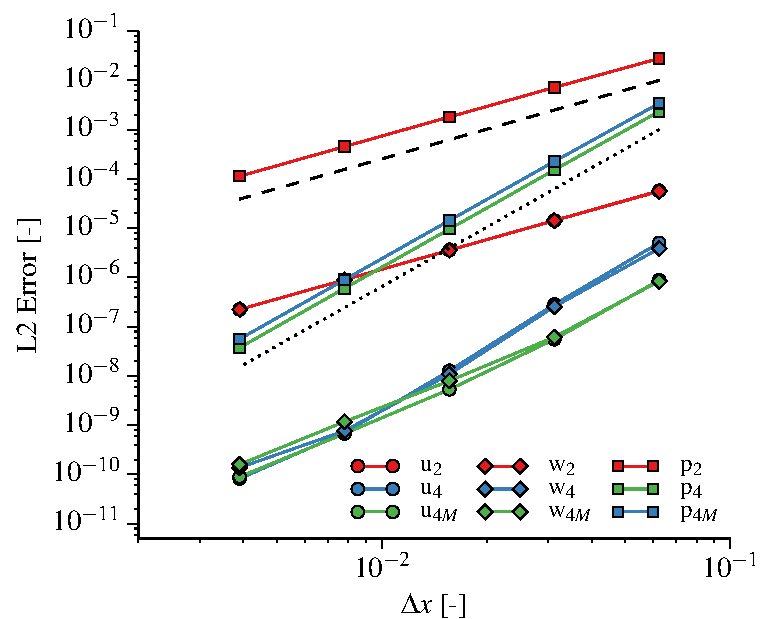
\includegraphics[width=8.3cm]{figs/taylorgreen.pdf}
	\end{center}
	\caption{Error convergence of the spatial discretization in the two-dimensional Taylor-Green vortex. The dashed black line shows second-order convergence, the dotted black line shows fourth-order convergence.}\label{fig:taylorgreen}
\end{figure}

Figure \ref{fig:taylorgreen} shows that the simulations have an excellent match with the analytical solution and the error converges according to the order of the scheme. The fourth-order dynamical core loses accuracy at fine grid spacings due to the treatment of the boundary condition for the vertical velocity that is constructed to ensure momentum conservation.

\subsection{Energy conservation and time accuracy} \label{sec:validationtime}
The second test of the dynamical core consist of combined evaluation of energy conservation and time accuracy (\texttt{cases/conservation}) . In this experiment, we switch the diffusion off and advect, using the energy-conserving fourth-order discretization, random noise through the domain for 1000 seconds. These tests have been done with the third- and fourth-order Runge-Kutta scheme.
\begin{figure}[t]
\vspace*{2mm}
\begin{center}
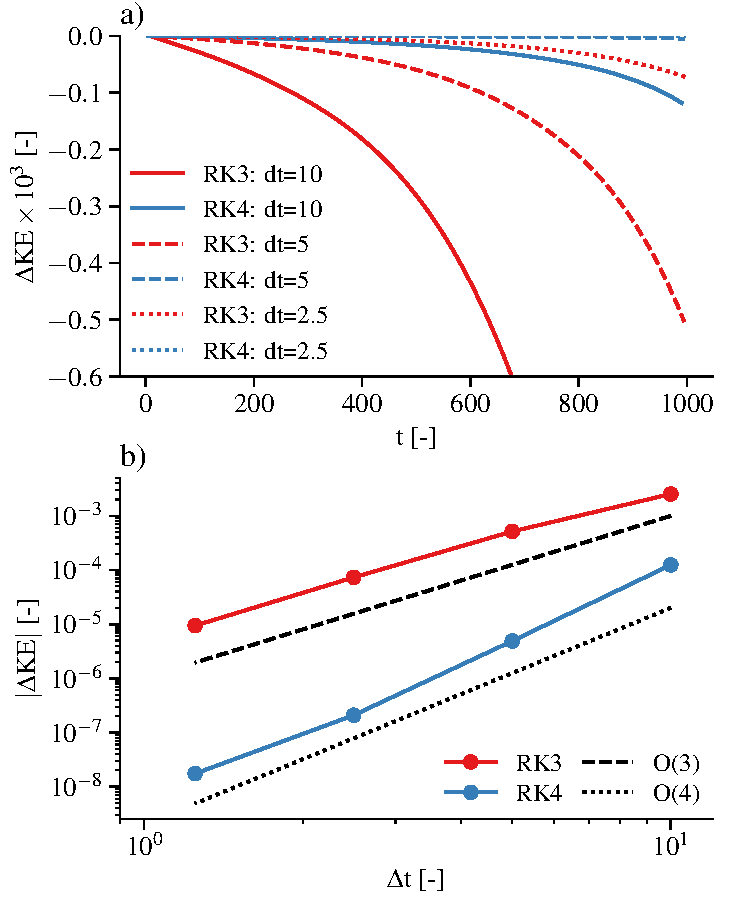
\includegraphics[width=8.3cm]{figs/timeconvergence.pdf}
\end{center}
\caption{Time evolution of the energy loss during 1000 time units of random noise advection for the RK3 and RK4 time integration schemes for three different time steps (a), and error convergence of the temporal discretization for the RK3 and RK4 scheme (b).}\label{fig:timeconvergence}
\end{figure}

The loss of energy as a function of time is shown in Figure \ref{fig:timeconvergence}a. The fourth-order scheme has a smaller energy loss for the same time step and converges faster. The error-convergence plot (Figure \ref{fig:timeconvergence}b) shows that the error convergence is in accordance with the respective scheme. Furthermore, it highlights that if high time accuracy is desired, the five-stage fourth-order scheme is less expensive than the three-stage third-order scheme. For instance, at a $\Delta t$ of 10, the L2 error of the fourth-order scheme is approximately equal to the L2 error of the third-order scheme at a $\Delta t$ of 2.5. To reach this accuracy the fourth-order scheme needs to take only 5 steps per 10 time units, whereas the third-order scheme has to take 12 steps.

\subsection{Laminar katabatic flow} \label{sec:laminarkatabatic}
To test the buoyancy routine and the option to put the surface under a slope, a laminar katabatic flow has been simulated, based on the test case of \citet{Prandtl1942} (\texttt{cases/prandtl}) . In this test case, the surface is put under an angle of $30^{\circ}$ and a linearly stratified atmosphere ($N = 1$~s$^{-1}$)  cooled from below with a fixed surface buoyancy flux of -0.005~m$^2$~$s^{-3}$.

\begin{figure*}[t]
	\vspace*{2mm}
	\begin{center}
		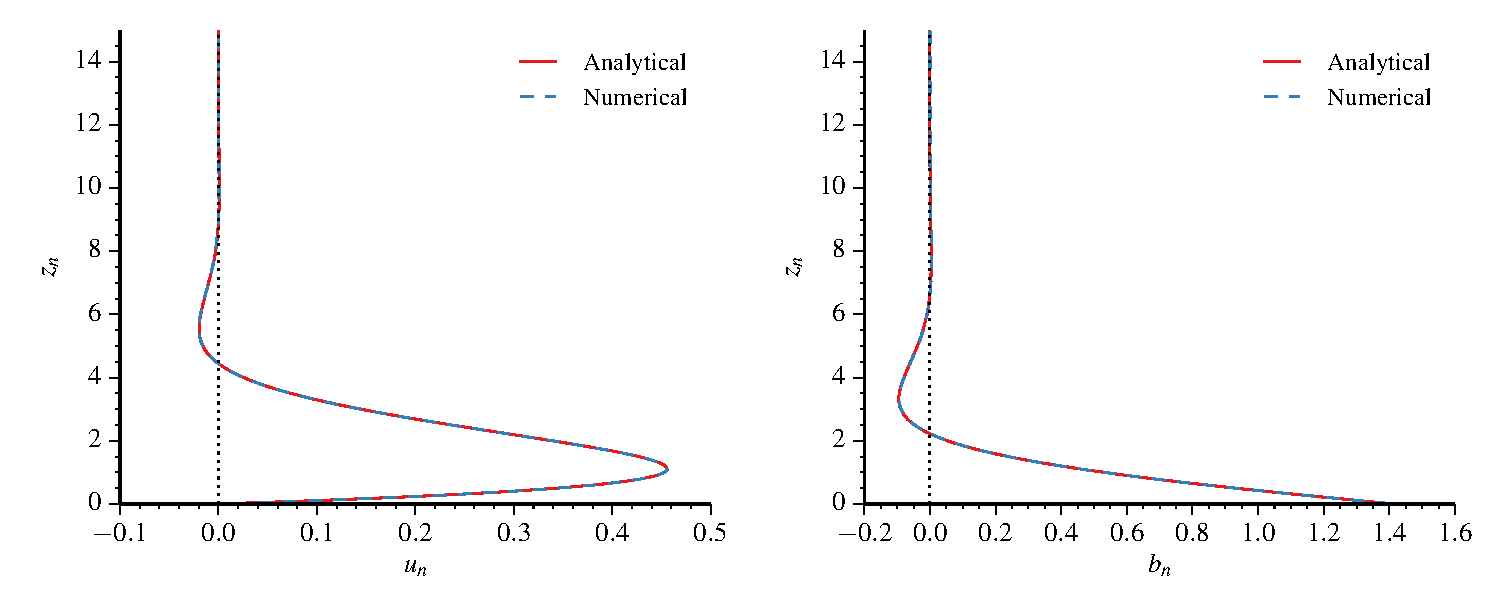
\includegraphics[width=16.6cm]{figs/prandtl.pdf}
	\end{center}
	\caption{Normalized numerical Prandtl-model solutions for velocity $u$ (left) and buoyancy $b$ (right) compared to their analytical counterparts.}
	\label{fig:prandtl}
\end{figure*}

The fluid, which was initially at rest, goes through a series of decaying oscillations after the negative buoyancy flux is applied at the surface. Eventually, it reaches the steady state corresponding to the Prandtl model solution. Numerical integration was performed sufficiently long for the oscillation amplitude to become a small fraction of the amplitude of the first oscillation. Comparison of analytical and numerical solutions, which very closely agree with each other, is presented in Fig.~\ref{fig:prandtl}.

\subsection{Turbulent channel flow}
For fully turbulent flows, the solution cannot be compared against an analytical testcase. Therefore, we validate our results against a channel flow at a Reynolds-$\tau$ number of 590 \citep{Moser1999} for means, variances, spectra and second order budget statistics (\texttt{cases/moser590}) .
\begin{figure}[t]
	\vspace*{2mm}
	\begin{center}
		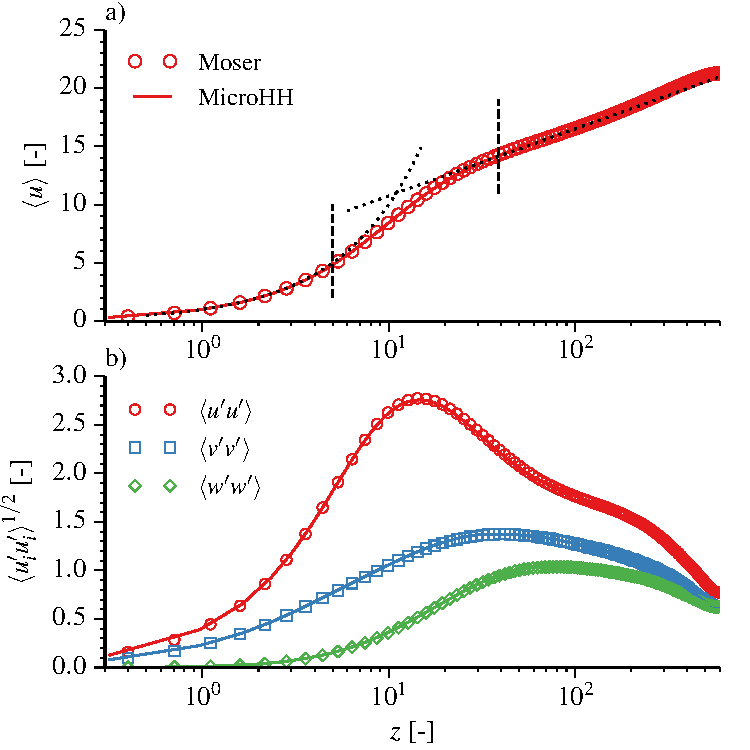
\includegraphics[width=8.3cm]{figs/gmd_m590_umean_var.pdf}
	\end{center}
	\caption{Velocity means and variances for \citet{Moser1999} channel flow case at Reynolds-$\tau$ 590. The dashed vertical lines marks the spectra locations. Height $z$ is normalized with $u_\tau / \nu$, velocities with $u_\tau^{-1}$.}\label{fig:moser_velocity}
\end{figure}

Figure \ref{fig:moser_velocity}a shows the normalized horizontally-averaged streamwise velocity in panel, and the normalized rms of all three velocity components in Figure \ref{fig:moser_velocity}b. All plotted variables show a perfect match with the data and are indistinguishable from Moser's data. In order to further assess the accuracy of the data, we show the second-order budgets of the variances in Figure \ref{fig:moser_budget}. Also here, the match with the reference data is excellent, which indicates that the whole range of spatial scales in the flow is represented well and that the fourth-order scheme is well able to pick up the small scale details of the flow.

The findings in the previous paragraph are further corroborated by the spectra shown in Figure \ref{fig:moser_spectra}.  Over the whole range of scales, the match between our simulation and that of Moser is excellent.


%% TWO-COLUMN FIGURES
\begin{figure*}[t]
\vspace*{2mm}
\begin{center}
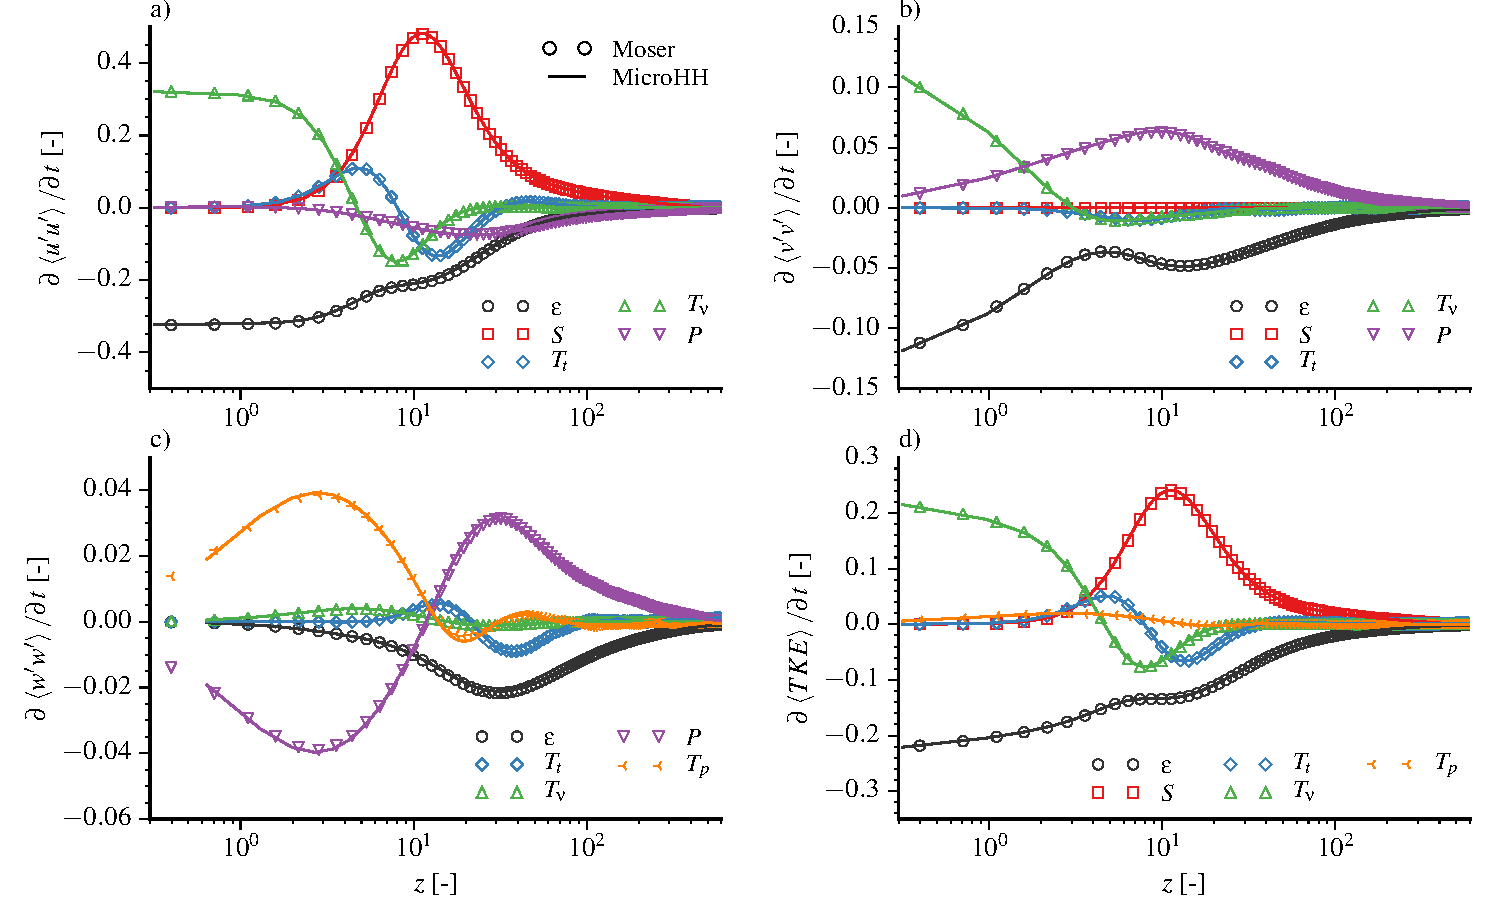
\includegraphics[width=16.6cm]{figs/gmd_m590_turb_budg.pdf}
\end{center}
\caption{Budgets of variances and TKE compared against \citet{Moser1999}'s reference data at Reynolds-$\tau$ of 590. Height $z$ is normalized with $u_\tau / \nu$, the variances and TKE budget with $\nu / u_\tau^{4}$.}\label{fig:moser_budget}
\end{figure*}

%% TWO-COLUMN FIGURES
\begin{figure*}[t]
\vspace*{2mm}
\begin{center}
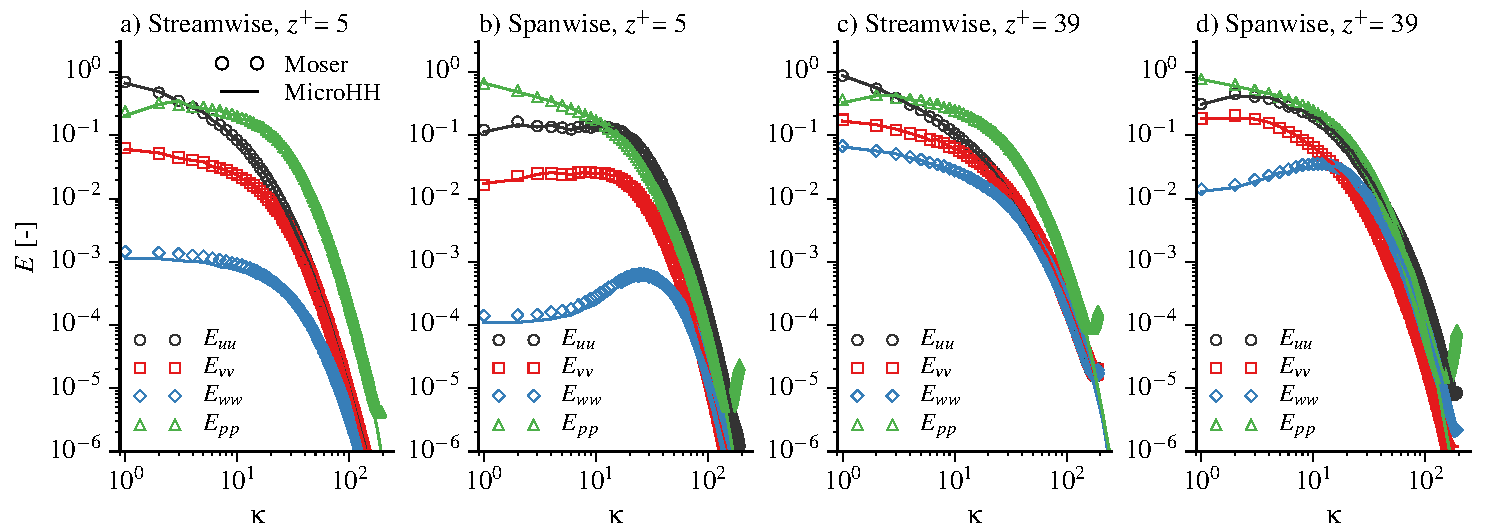
\includegraphics[width=16.6cm]{figs/gmd_m590_spectra_4x1.pdf}\label{fig:moser_spectra}
\end{center}
\caption{Spectra of all velocity components and pressure compared against \citet{Moser1999}'s reference data at Reynolds-$\tau$ of 590. The velocity spectra are normalized with $u_\tau^{-2}$, the pressure spectra with $u_\tau^{-4}$}
\end{figure*}

\subsection{Turbulent katabatic flow}
\subsubsection{Simulation settings}
\begin{itemize}
	\setlength{\itemsep}{0pt}
	\setlength{\parskip}{0pt}
	\setlength{\parsep}{0pt}  
	\item Slope angle: $\alpha = 60^{\circ}$
	\item Surface buoyancy flux: $B_{s} $ = $-0.5{\rm\, m}^{\rm 2}\, {\rm s}^{{\rm -3}} $
	\item Brunt-V\"{a}is\"{a}l\"{a} (buoyancy) frequency: $N$ = $1\,{\rm s}^{{\rm -1}}$
	\item Kinematic viscosity/thermal diffusivity:\\$\nu$ = $-0.0001{\rm\, m}^{\rm 2}\, {\rm s}^{{\rm -1}} $
	\item Domain size: ($X{\times}Y{\times}Z$) = 0.64${\rm\, m}\times$0.64${\rm\, m}\times$1.6${\rm\, m}$
	\item Numerical grid dimensions: \\($n_x{\times}n_y{\times}n_z$) = $256 \times 256 \times 640$
	\item Grid structure: uniform (non-stretched) grid in all three directions, with $\Delta x = \Delta y = \Delta z$ = 0.0025${\rm\, m}$
	\item Time step: adaptive
	\item Initial condition: stratified fluid at rest above the slope with zero surface buoyancy flux
	\item Lateral boundary conditions: periodic
	\item Lower boundary conditions: no-slip and impermeability conditions for velocity, surface-flux condition for buoyancy
	\item Upper boundary conditions: free-slip conditions for velocity, zero-gradient condition for buoyancy
\end{itemize}

\subsubsection{Flow description and simulation results}
The final evaluation of the dynamical core without parametrizations enabled is based on a turbulent katabatic flow. Here, a buoyancy driven slope flow is simulated following the setup of \citet{Fedorovich2009} (\texttt{cases/drycblslope}).

Turbulent motion starts quickly after the buoyancy flux is applied at the surface. It is characterized by random, large-amplitude fluctuations of velocity and buoyancy fields in the near-slope core region and shows a quasi-periodic oscillatory behavior at larger distances from the slope. Mean profiles of along-slope velocity component and buoyancy, as well as profiles of second-order turbulence statistics, such as kinematic turbulent fluxes of momentum and buoyancy, and velocity-component and buoyancy fluctuation variances, were evaluated by averaging the simulated flow fields spatially over $xy$-planes and temporally over five oscillation periods beyond the transition stage.

For comparison, the same katabatic flow case was reproduced using the numerical code (hereafter referred to FS09) that was employed to simulate turbulent slope flows in \citet{Shapiro2008} and \citet{Fedorovich2009}. In the version of the code used in this comparison study, the time advancement was performed with an Asselin-filtered second-order leapfrog scheme \citep{Durran2013}. The spatial discretizations are identical to the second-order accurate ones of MicroHH. No-slip and impermeability conditions are applied on the velocity field at the slope surface. Normal gradients of prognostic variables (velocity components and buoyancy) are set to zero at the outer computational boundary, and periodic boundary conditions are imposed at the $xz$- and $yz$-boundaries of the computational domain.

Numerical results obtained with both numerical codes testify that stable environmental stratification in combination with negative surface buoyancy forcing in the katabatic flow leads to an effective suppression of vertical turbulent exchange in the flow region adjacent to the slope. This suppression results in a shallow near-surface sublayer with strong buoyancy gradients (Figure~\ref{katabatic_b}) capped by a narrow mean-velocity jet with peak velocity located very close to the ground. (Figure~\ref{katabatic_u}).

\begin{figure}
	\centerline{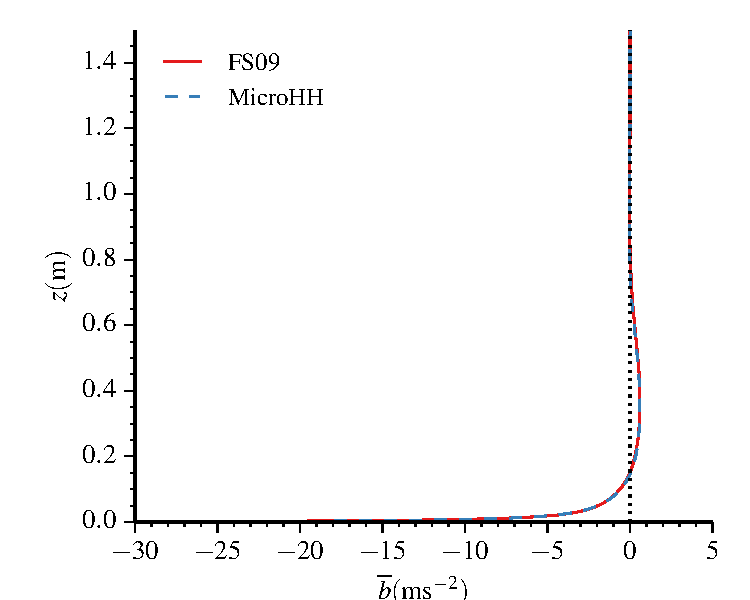
\includegraphics[width=8.3cm]{figs/katabatic_b.pdf}}
	\caption{Profile of the mean buoyancy as predicted by MicroHH and FS09.}
	\label{katabatic_b}
\end{figure}

\begin{figure}
	\centerline{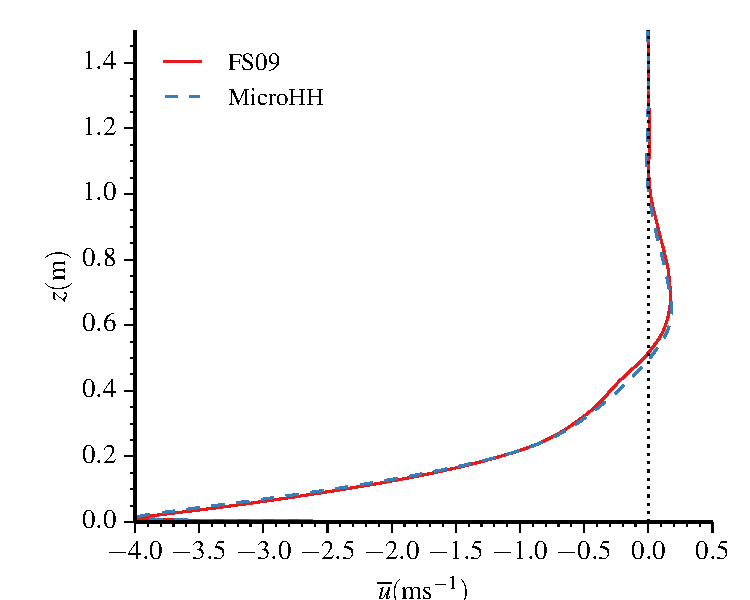
\includegraphics[width=8.3cm]{figs/katabatic_u.pdf}}
	\caption{Profile of the mean along-slope velocity as predicted by MicroHH and FS09.}
	\label{katabatic_u}
\end{figure}

As revealed by the buoyancy variance profiles in (Fig.~\ref{katabatic_bb}), the buoyancy fluctuations in the simulated katabatic flow attain their maximum magnitude extremely close to the wall, roughly within the region where maximum gradients are observed in the mean buoyancy profiles (Fig.~\ref{katabatic_b}). The drop of $\overline{b'b'}$ beyond the maximum is also rather sharp which means that significant fluctuations of the buoyancy are restricted to a comparatively thin near-wall sublayer.

\begin{figure}
	\centerline{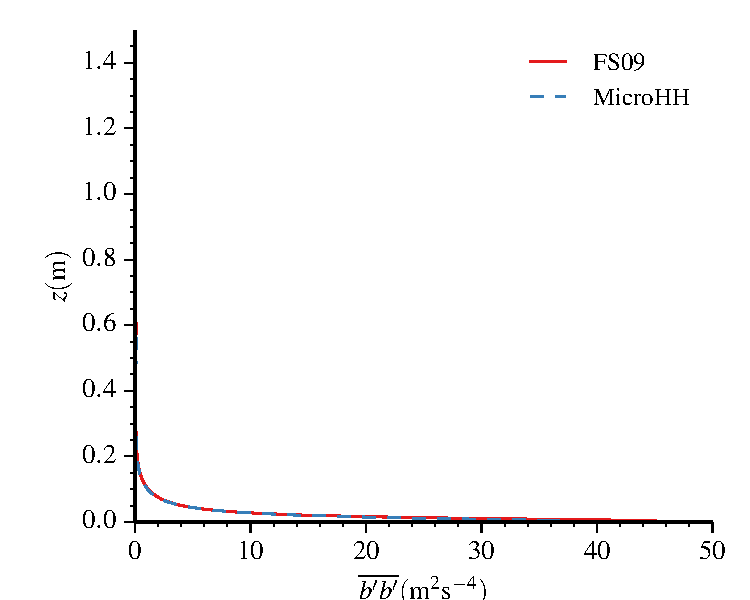
\includegraphics[width=8.3cm]{figs/katabatic_bb.pdf}}
	\caption{Profile of the buoyancy variance as predicted by MicroHH and FS09.}
	\label{katabatic_bb}
\end{figure}

Along-slope velocity fluctuations of notable magnitudes are distributed over the layer that is about four times thicker than the layer which contains most of the buoyancy variance (compare Fig.~\ref{katabatic_uu} and Fig.~\ref{katabatic_bb}). While the two codes agree with respect to predicting the overall behavior of $\overline{u'u'}$, MicroHH predicts a smoother and stronger maximum of the velocity variance than FS09. The magnitudes of the maxima, though, are fairly close to each other in Fig.~\ref{katabatic_uu}.

\begin{figure}
	\centerline{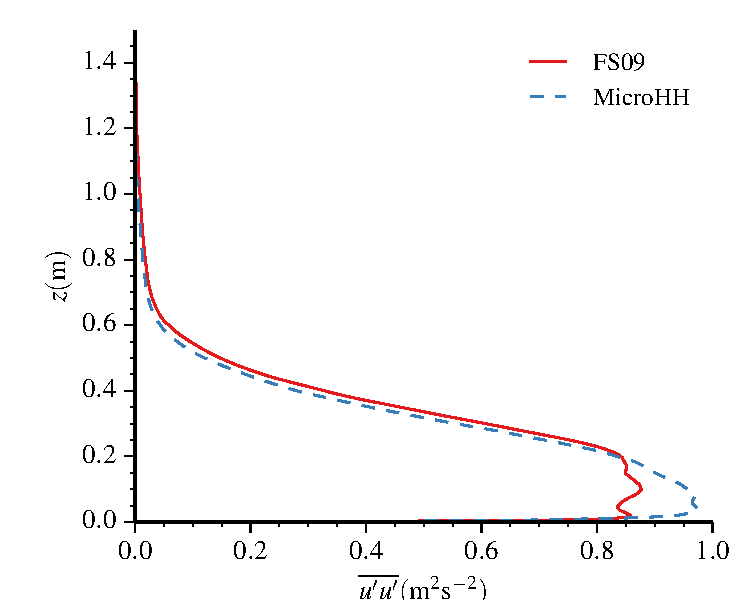
\includegraphics[width=8.3cm]{figs/katabatic_uu.pdf}}
	\caption{Profile of the along-slope velocity variance as predicted by MicroHH and FS09.}
	\label{katabatic_uu}
\end{figure}

Comparisons of profiles of the cross-slope velocity component variance, $\overline{v'v'}$, and the slope-normal component variance, $\overline{w'w'}$, are presented in Fig.~\ref{katabatic_vv} and Fig.~\ref{katabatic_ww}, respectively.

\begin{figure}
	\centerline{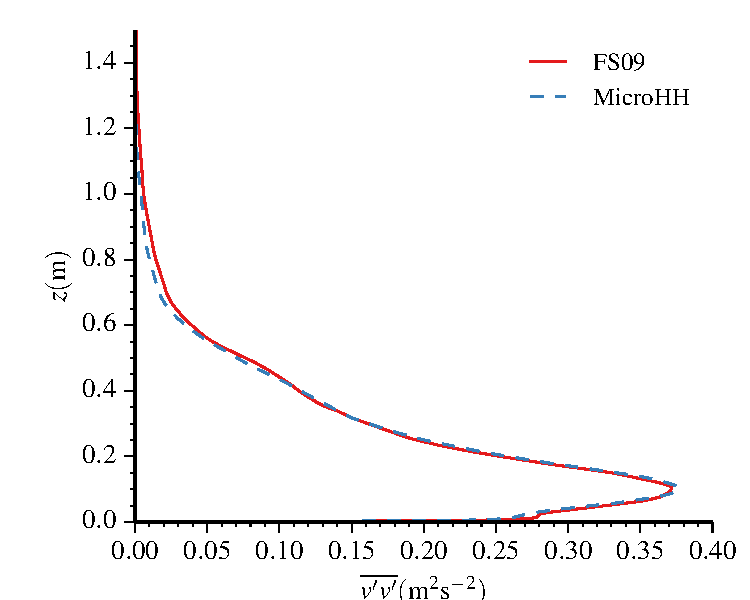
\includegraphics[width=8.3cm]{figs/katabatic_vv.pdf}}
	\caption{Profile of the cross-slope velocity variance as predicted by MicroHH and FS09.}
	\label{katabatic_vv}
\end{figure}

\begin{figure}
	\centerline{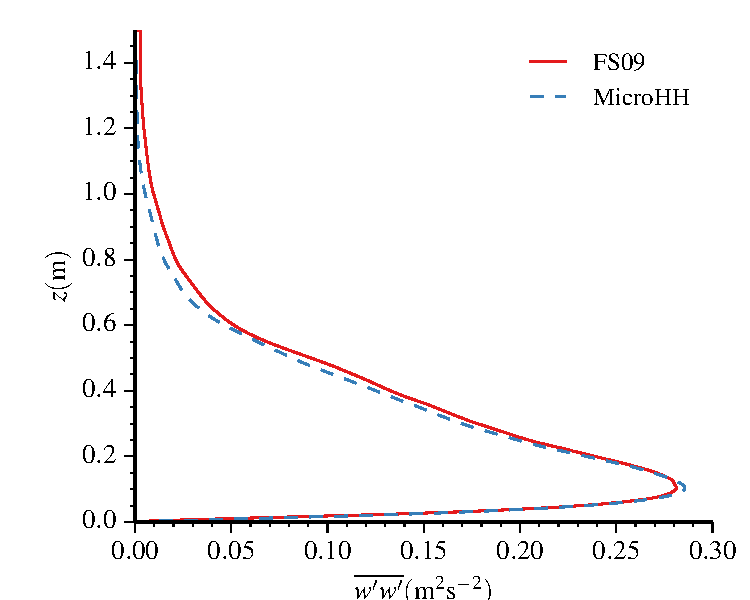
\includegraphics[width=8.3cm]{figs/katabatic_ww.pdf}}
	\caption{Profile of the slope-normal velocity variance as predicted by MicroHH and FS09.}
	\label{katabatic_ww}
\end{figure}

Profiles of slope-normal fluxes of momentum, $\overline{w'u'}$ (Fig.~\ref{katabatic_wu}), and buoyancy, $\overline{w'b'}$ (Fig.~\ref{katabatic_wb}), indicate that zero crossings in the mean profiles of \textit{b} and \textit{u} are closely co-located with the minima and maxima of the fluxes $\overline{u'w'}$ and $\overline{b'w'}$ except for locations very close to the wall, where molecular effects are important. Typically, molecular fluxes in the simulated flows become negligible at distances from the surface that are significantly smaller than the elevation of the mean velocity maximum (jet elevation).

\begin{figure}
	\centerline{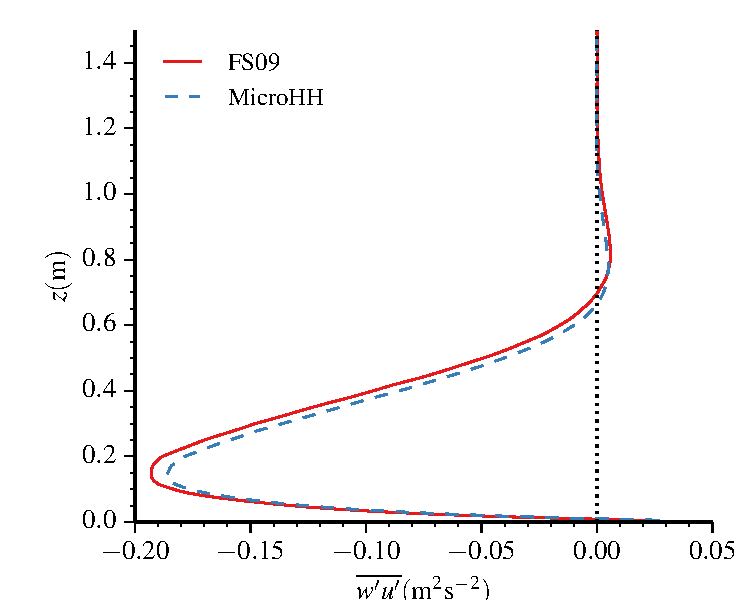
\includegraphics[width=8.3cm]{figs/katabatic_wu.pdf}}
	\caption{Profile of the slope-normal turbulent kinematic momentum flux as predicted by MicroHH and FS09.}
	\label{katabatic_wu}
\end{figure}

\begin{figure}
	\centerline{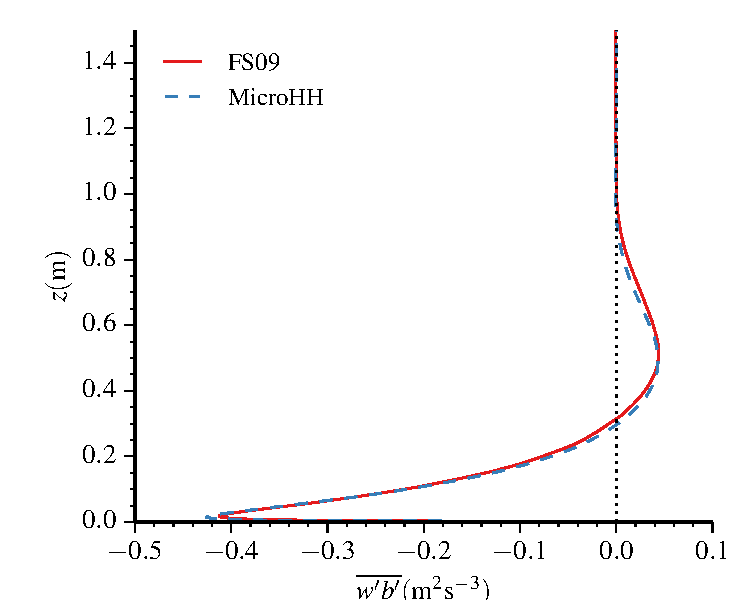
\includegraphics[width=8.3cm]{figs/katabatic_wb.pdf}}
	\caption{Profile of the slope-normal turbulent kinematic buoyancy flux as predicted by MicroHH and FS09.}
	\label{katabatic_wb}
\end{figure}

Flux profiles shown in Fig.~\ref{katabatic_wu} and Fig.~\ref{katabatic_wb} indicate that there is no region in the flow domain with constancy (even approximate) of either flux with distance from the wall. In more conventional boundary-layer type flows, the existence of height intervals with slowly changing (in the first approximation, constant) momentum and buoyancy fluxes is used as a foundation for similarity analyses and scalings. Such a constant-flux formalism does not apply, at least in a straightforward manner, to the considered katabatic flow case.

\subsection{BOMEX}

To validate the moist thermodynamics (influence of phase changes on buoyancy) Fig. \ref{fig:bomex} shows the comparison of MicroHH for the BOMEX non-precipitating shallow cumulus LES intercomparison (SIEBESMA), using the resolution from the intercomparison setup (100 m $\times$ 100 m $\times$ 40 m) and a higher resolution (10 m $\times$ 10 m $\times$ 9.375 m) setup. All mean and conditionally sampled statistics are predominantly within one standard deviation of the results from SIEBESMA, except for the cloud and cloud core vertical velocity in the higher resolution setup (STILL LOOKING INTO WHY, T.B.C...). 

\begin{figure*}[t]
\vspace*{2mm}
\begin{center}
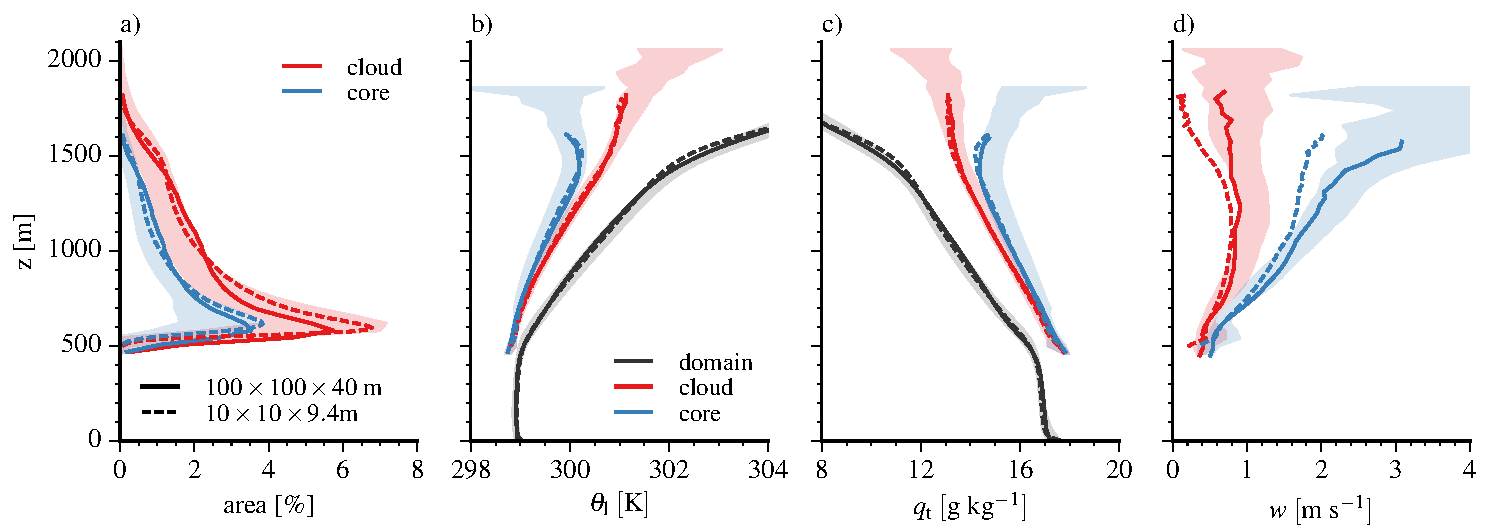
\includegraphics[width=16.6cm]{figs/gmd_bomex_profs.pdf}
\end{center}
\caption{BOMEX LES intercomparison (SIEBESMA). Shown are the domain mean, and conditionally sampled cloud ($q_\mathrm{l} > 0$) and cloud core ($q_\mathrm{l}>0 \ \mathrm{and} \ b-\langle b \rangle > 0$) vertical profiles of (a) area coverage, (b) liquid water potential temperature, (c) total specific humidity and (d) vertical velocity. The results are averaged over t=18000 s -- 21600 s. The shaded area denotes the mean $\pm$ one standard deviation of the participating models from SIEBESMA, the solid and dashed lines the results from MicroHH, using the original (solid) and a higher resolution (dashed) setup.}
\label{fig:bomex}
\end{figure*}

\subsection{GABLS1}
To validate the Large-Eddy Simulation mode under stable conditions, results for the GABLS1 LES intercomparison case \citep{Beare2006} are shown (\texttt{cases/gabls1}). The result from MicroHH were obtained using the Boussinesq approximation, a centered advection scheme with 4th order accurate interpolations (SECOND ORDER ADVECTION WITH HIGHER ORDER INTERPOLATIONS IS NOT YET DESCRIBED...), and Smagorinsky diffusion using $C_\mathrm{s}$ = 0.XX and a turbulent Prandtl number of XX (JUST TO BE SURE I'LL RE-RUN THESE EXPERIMENTS, RESULTS ARE REALLY OLD...)

\begin{figure*}[t]
\vspace*{2mm}
\begin{center}
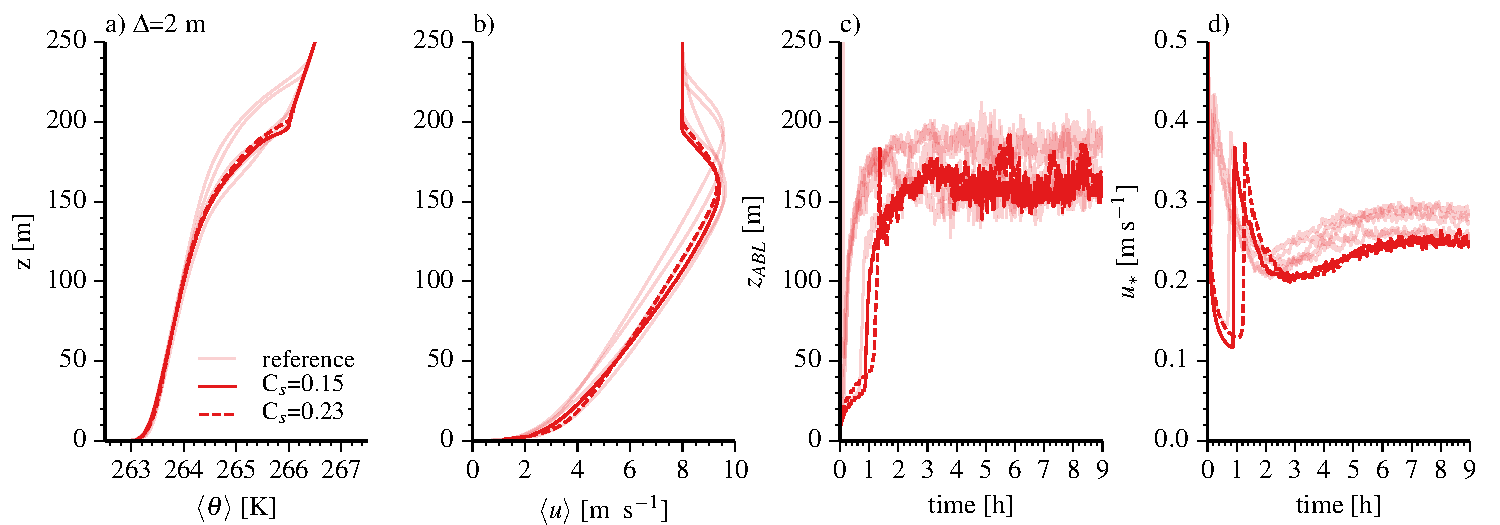
\includegraphics[width=16.6cm]{figs/gmd_gabls_prof_tser.pdf}
\end{center}
\caption{GABLS1 LES intercomparison \citep{Beare2006}. Shown are the vertical profiles of (a) potential temperature and (b) u-component of the horizontal velocity, and time series of the (c) boundary layer depth and (d) surface friction velocity. The vertical profiles are averages over t=28800 s -- 32400 s. In gray the results from the participating models from  \citep{Beare2006} (2~m resolution) are shown, in blue and red the results from MicroHH using a 2 m and 6.25 m grid spacing, respectively. The dotted black line shows the initial conditions.}
\label{fig:gabls}
\end{figure*}

\section{Performance}\label{sec:performance}
\subsection{CPU}
\begin{figure}[!hbt]
	\vspace*{2mm}
	\begin{center}
		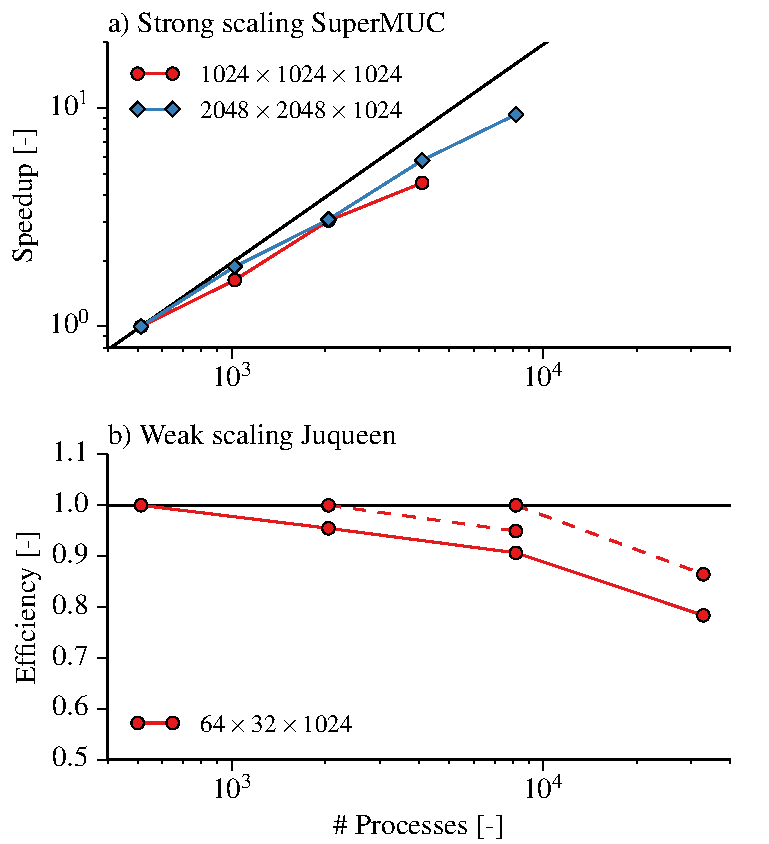
\includegraphics[width=8.3cm]{figs/scaling.pdf}
	\end{center}
	\caption{Bla?}\label{fig:scaling}
\end{figure}
The parallel performance of MicroHH has been evaluated in strong and weak scaling experiments. We have chosen a buoyancy driven direct numerical simulation as a reference case, based on \citet{vanHeerwaarden2014}. For each simulation in the scaling experiments, a series of time steps is performed and the mean cost per step is calculated over the series. The strong scaling experment has been performed on LRZ's SuperMUC\footnote{\url{https://www.lrz.de/services/compute/supermuc/}} machine. In this experiment simulations were done on grids of respectively $1024 \times 1024 \times 1024$ and $2048 \times 2048 \times 1024$ grid points, where the number of processes is increased throughout the scaling experiment. The weak scaling experiment has been performed on Forschungszentrum J\"{u}lich's Juqueen\footnote{\url{http://www.fz-juelich.de/ias/jsc/EN/Expertise/Supercomputers/JUQUEEN/JUQUEEN_node.html}} machine. Within this experiment a fixed grid size of $64 \times 32 \times 1024$ grid points is assigned to each processor and throughout the experiment the domain size is increased. The results of both experiments are shown in Figure \ref{fig:scaling}.

The strong scaling experiments show that increasing the number of processors leads to faster simulations. The speedup is following the linear line, but each consecutive increase in the number of cores makes the model less efficient. Based on these results, we conclude that for the chosen test case, a work load of approximately $2\cdot 10^6$ grid points per core is the best balance between speed and computational efficiency.

The weak scaling shows almost 90 percent efficiency going from 512 to 8192 cores, beyond that the scaling falls off to 80 percent. This can be explained by physical properties of the machine;  beyond 8192 cores a simulation no longer fits on one midplane (with 8192 cores), leading to slower communication.

\subsection{Performance GPU (CUDA) implementation}
The GPU implementation of MicroHH allows for fast computations on a single core. The state-of-the-art GPU at the time of these benchmarks feature 6~GB of memory. With the memory efficiency of MicroHH this allows for simulations up to $512 \times 512 \times 384$ for a flow with three velocity components and a single scalar. To test the performance of the code, the performance of a single NVIDIA Quadro K6000 (Cuda 6.5) has been compared against the Max Planck Institute for Meteorology's cluster Thunder (2 Intel Xeon E5-2670 CPU's per node, 16 cores per node, Intel 15.01 with OpenMPI 1.8.4). Three benchmark cases have been chosen: the BOMEX moist convection case at grid dimensions of $64^3$, $128^3$, $256^3$ and $512^2 \times 384$ and the channel flow cases of \citet{Moser1999} at a Reynolds-$\tau$ number of 180 and 590.

\begin{table}[t]
	\caption{Speedup of GPU simulation compared to respective CPU simulation performed on $n$ cores.}\label{tab:gpu}
	\begin{tabular}{rccccc}
		\tophline
		case & $n$=1 & $n$=16 & $n$=32 & $n$=64   \\
		\middlehline
		B64  & 18.49 & 1.93 & 1.14 & 0.95 \\
		B128 & 28.01 & 2.98 & 1.51 & 0.92 \\
		B256 & 27.76 & 3.02 & 1.59 & 0.91 \\
		B512 & 29.88 & 3.03 & 1.56 & 0.86 \\
		\middlehline
		M180 & 21.57 & 2.17 & 1.13 & 0.69 \\
		M600 & 22.55 & 2.25 & 1.06 & 0.60 \\
		\bottomhline
	\end{tabular}
\end{table}

The results shown in Table \ref{tab:gpu} show the great potential of GPU computing. For these cases, that all fit on a single GPU, it takes at least 32 cores to reach equal performance. Only at 64 cores, the CPU simulations are notably faster. Therefore, for simulations that fit into its memory, the GPU provides an excellent alternative for the CPU.

\section{Future plans}
Currently, there are several ongoing projects to extend the model. The physical processes at are currenlty being implemented are microphysics and an interactive land surface model. [BART] Furthermore, immersed boundaries are being implemented to allow for simulation of flow over obstacles and hills.

Furthermore, preliminary experiments have been performed to include a Domain-Specific Language (DSL) that enables the expression of complex finite difference operators in a simple syntax. The project has shown great potential, for two reasons. First, the DSL reduces the chances of making errors, as the explicit indexing in computational kernels with spatial operators can be omitted. Second, the DSL allows for simple implementation of system specific tuning, such as loop tiling or OpenMP.

\conclusions  \label{sec:conclusion} %% \conclusions[modified heading if necessary]
This paper presents a full description MicroHH, an new Computational Fluid Dynamics code for simulations of turbulent flows in the atmospheric boundary layer. The governing equations and their implementation has been presented, and a broad validation under a wide range of settings has been shown.

\section{Availability of code and resources}
MicroHH has its own website at \url{http://microhh.org}. Its code is hosted at GitHub and can be accessed either via the website, or directly from 
\url{https://github.com/microhh/microhh}. A selection of visualizations can be viewed at the MicroHH channel at Vimeo \url{https://vimeo.com/channels/817195}.

\iffalse
\section{Appendix}
\begin{table*}[t]
\caption{Overview of used symbols}\label{tab:symbols}
\begin{tabular}{lll}
\tophline
Symbol & Description & Units \\
\middlehline
$\rho_0$ & Reference density & kg~m$^{-3}$\\
$H_\rho$ & Scale height for density & m\\
$u_i$  & Velocity vector $\left( u, v, w \right)$ & m~s$^{-1}$\\
$x_i$  & Position vector $\left( x, y, z \right)$ & m\\
$p^\prime$ & Perturbation pressure & Pa\\
$p_0$ & Reference pressure & Pa\\
$\rho^\prime$ & Perturbation density & kg~m$^{-3}$ \\
$p^\prime$ & Perturbation pressure & Pa\\
$p_0$ & Reference pressure & Pa\\
$\theta_v^\prime$ & Perturbation virtual potential temperature & K\\
$\theta_{v0}$ & Reference virtual potential temperature & K\\
$g$ & Gravity acceleration & m~s$^{-2}$\\
$\nu$ & Kinematic viscosity & m$^{2}$~s$^{-1}$\\
$\kappa$ & Scalar diffusivity & m$^{2}$~s$^{-1}$\\
$F_i$ & External acceleration vector &  m~s$^{-2}$\\
$S$ & External sources and sinks & variable dependent\\
$\theta$ & Potential temperature & K \\
$\theta_l$ & Liquid water potential temperature & K\\
$b$ & Buoyancy & m~s$^{-2}$\\
$T_0$ & Reference absolute temperature & K\\
$Q$ & Heat input & J~m$^{-3}$~s$^{-1}$\\
$\alpha$ & Slope of surface & rad \\
$N$ & Brunt-Vaissala frequency & s\\
\bottomhline
\end{tabular}
\end{table*}
\fi

\bibliographystyle{copernicus}
\bibliography{../../misc/refs}
%\bibliography{microhharticle}

\end{document}
